\documentclass[11pt,a4paper]{article}
\usepackage[margin=2.6cm]{geometry}
\usepackage[T1]{fontenc}
\usepackage{lmodern}
\usepackage{amsmath,amssymb,amsthm}
\usepackage{bm}
\usepackage{graphicx}
\usepackage{booktabs}
\usepackage{xcolor}
\usepackage[colorlinks=true,linkcolor=blue!50!black,citecolor=blue!50!black,urlcolor=blue!50!black]{hyperref}

\graphicspath{{figures/}}
\setlength{\parskip}{0.35em}
\numberwithin{equation}{section}

\theoremstyle{plain}
\newtheorem{proposition}{Proposition}[section]
\newtheorem{lemma}[proposition]{Lemma}
\newtheorem{theorem}[proposition]{Theorem}
\newtheorem{corollary}[proposition]{Corollary}
\theoremstyle{definition}
\newtheorem{definition}[proposition]{Definition}
\newtheorem{example}[proposition]{Example}
\newtheorem{procedure}[proposition]{Algorithm}
\theoremstyle{remark}
\newtheorem{remark}[proposition]{Remark}

% ---------------------------------------------------------------- notation
\newcommand{\m}{\mathbf{m}}
\newcommand{\z}{\mathbf{z}}
\newcommand{\x}{\mathbf{x}}
\newcommand{\y}{\mathbf{y}}
\newcommand{\uu}{\mathbf{u}}
\newcommand{\e}{\mathbf{e}}
\newcommand{\rr}{\mathbf{r}}
\newcommand{\vv}{\mathbf{v}}
\newcommand{\aaa}{\mathbf{a}}
\newcommand{\bb}{\mathbf{b}}
\newcommand{\eps}{\bm{\varepsilon}}
\newcommand{\thetab}{\bm{\theta}}
\newcommand{\zetab}{\bm{\zeta}}
\newcommand{\mub}{\bm{\mu}}
\newcommand{\Sig}{\bm{\Sigma}}
\newcommand{\Lb}{\mathbf{L}}
\newcommand{\Cb}{\mathbf{C}}
\newcommand{\Ab}{\mathbf{A}}
\newcommand{\Pb}{\mathbf{P}}
\newcommand{\Qb}{\mathbf{Q}}
\newcommand{\I}{\mathbf{I}}
\newcommand{\Sset}{\mathcal{S}}
\newcommand{\E}{\mathbb{E}}
\newcommand{\R}{\mathbb{R}}
\newcommand{\Var}{\mathrm{Var}}
\newcommand{\Cov}{\mathrm{Cov}}
\newcommand{\tr}{\mathrm{tr}}
\newcommand{\KL}{\mathrm{KL}}
\newcommand{\Hent}{\mathrm{H}}
\newcommand{\ELBO}{\mathrm{ELBO}}
\newcommand{\NLL}{\mathrm{NLL}}
\newcommand{\MAC}{\mathrm{MAC}}
\newcommand{\Lc}{\mathcal{L}}
\newcommand{\N}{\mathcal{N}}
\newcommand{\U}{\mathcal{U}}
\newcommand{\Dc}{\mathcal{D}}
\newcommand{\dd}{\,\mathrm{d}}
\newcommand{\zlb}{z_{\text{lb}}}
\newcommand{\zub}{z_{\text{ub}}}
\newcommand{\Ntr}{N_{\text{train}}}
\newcommand{\qth}{q_{\bm{\theta}}}
\newcommand{\ind}{\mathbb{I}}

\title{Bayesian posterior estimation in inverse problems\\with variational autoencoders\\[0.4em]
\large From the basic probability tools to the physics-informed copula VAE\\
Background notes for the CPENG-8674 revision}
\author{}
\date{November 2026}

\begin{document}
\maketitle

\begin{abstract}
These notes develop, from first principles, the theory behind the loss function of the physics-informed copula VAE of the revised CPENG-8674 manuscript. They are general enough to serve as a background on Bayesian inference and variational inference for inverse problems, and specific enough to explain every term of the loss.
Part~\ref{part:tools} collects and proves the probability tools used later.
Part~\ref{part:bayes} formulates the Bayesian inverse problem: how the error model determines the likelihood, the prior, the posterior and the evidence, with worked examples solved step by step.
Part~\ref{part:vi} introduces the entropy, the Kullback--Leibler divergence, variational inference and the evidence lower bound (ELBO), amortized inference with an encoder (the VAE), the reparameterization trick and the temperature $\gamma$.
Part~\ref{part:loss} starts from the loss function of the original formulation (as written in the published copula-VAE paper on floating offshore wind turbines and as implemented for the submitted CPENG-8674 manuscript), computes which posterior it actually estimated, and derives the loss of the revised manuscript.
Part~\ref{part:families} describes the posterior families: the probability integral transform, Sklar's theorem, the Gaussian copula, and the truncated Gaussian, truncated log-normal, truncated Gaussian-mixture and Kumaraswamy-mixture marginals, with their densities, CDFs, inverse CDFs, entropies, means and sampling algorithms.
\end{abstract}

\tableofcontents

% =====================================================================================================
\section*{How to read these notes and notation}
\addcontentsline{toc}{section}{How to read these notes and notation}

Every statement is derived in the notes, with two exceptions, which are standard results of calculus and linear algebra and are stated explicitly where they are used: the change of variables in multiple integrals (Theorem~\ref{thm:cov_multi}) and the basic properties of determinants, traces and eigenvalues (Section~\ref{sec:linalg}).
Each section uses only the results of the previous ones.
A reader who knows basic probability can skim Part~\ref{part:tools} and come back to it when a result is cited.
The notation follows the revised manuscript (Table~\ref{tab:notation}).

\begin{table}[h]
\centering
\caption{Notation.}
\label{tab:notation}
\small
\begin{tabular}{@{}lp{9.2cm}@{}}
\toprule
Symbol & Meaning \\
\midrule
$\z=(z_1,\dots,z_D)$ & stiffness factors (unknowns, latent variables); $D=7$ (5 deck zones, 2 bearings) \\
$\Sset=[\zlb,\zub]^D$ & support of $\z$ (prior box); $\zlb=0.45$, $\zub=1$ \\
$\z^{\text{true}}$ & true damage condition of a scenario \\
$\m=\{\mathbf{f},\bm{\Phi}\}$ & observation: natural frequencies $\mathbf{f}\in\R^{n_m}$ and mode shapes $\bm\Phi\in\R^{n_m\times n_s}$ \\
$\Dc(\z)=\{\hat{\mathbf f}(\z),\hat{\bm\Phi}(\z)\}$ & forward model (decoder): FE model and eigenvalue problem \\
$\eps$ & error: difference between the observation and the forward model \\
$p(\z)$, $p(\m|\z)$, $p(\z|\m)$, $p(\m)$ & prior, likelihood, posterior, evidence \\
$\NLL(\z;\m)$ & negative log-likelihood, $-\log p(\m|\z)$ (up to a constant) \\
$\qth(\z|\m)$ & approximate posterior given by the encoder with weights $\thetab$ \\
$\zetab(\thetab)$ & parameters of $\qth$ output by the encoder \\
$q_d,F_d,F_d^{-1}$ & marginal density, CDF and inverse CDF of $z_d$ under $\qth$ \\
$\varphi,\Psi$ & standard normal density and CDF ($\bm\Phi$ is reserved for the mode shapes) \\
$\Sig=\Lb\Lb^\top$ & correlation matrix of the Gaussian copula, $\Lb$ lower triangular \\
$\Hent[q]$, $\KL(q\,\|\,p)$ & entropy, Kullback--Leibler divergence \\
$\gamma$ & temperature (weight of the entropy term) \\
$H$, $\Ntr$ & samples per observation in the loss; number of training observations \\
$\ind_A(\x)$ & indicator function: 1 if $\x\in A$, 0 otherwise \\
\bottomrule
\end{tabular}
\end{table}

Conventions: (i) the loss is the \emph{negative} ELBO: training minimizes the loss and maximizes the ELBO; (ii) ``constant'' means ``independent of $\z$ and of the encoder weights $\thetab$''; such terms change neither the minimizer nor the gradients; (iii) $\log$ is the natural logarithm.

% =====================================================================================================
\part{Probability toolkit}
\label{part:tools}

\section{Random variables, densities and expectations}
\label{sec:tools}

\subsection{Densities and cumulative distribution functions}
A continuous random variable $X$ is described by its \emph{probability density function} (PDF) $p(x)\ge0$, which gives probabilities of intervals by integration:
\begin{equation}
P(a<X\le b)=\int_a^bp(x)\dd x,\qquad \int_{-\infty}^{\infty}p(x)\dd x=1.
\end{equation}
The \emph{cumulative distribution function} (CDF) is $F(x)=P(X\le x)=\int_{-\infty}^xp(t)\dd t$. It is non-decreasing, goes from 0 to 1, and, by the fundamental theorem of calculus, $F'(x)=p(x)$.
Hence $P(a<X\le b)=F(b)-F(a)$.
If $F$ is strictly increasing on the set where $p>0$, it has an inverse $F^{-1}:(0,1)\to\R$, the \emph{quantile function}: $F^{-1}(u)$ is the value below which $X$ falls with probability $u$.
For a random vector $\x=(x_1,\dots,x_D)$, $p(\x)$ is the joint density, and $P(\x\in A)=\int_Ap(\x)\dd\x$.

A density can exceed 1 (it is a probability \emph{per unit length}); only its integral must be 1. Example: the uniform density on $[0,0.1]$ equals 10.

\subsection{Expectations, variances and covariances}
The expectation of a function $g$ of $X$ is
\begin{equation}
\E[g(X)]=\int g(x)\,p(x)\dd x.
\label{eq:lotus}
\end{equation}
Equation~\eqref{eq:lotus} is consistent with the definition $\E[Y]=\int y\,p_Y(y)\dd y$ of the variable $Y=g(X)$: for a strictly monotone $g$, the substitution $y=g(x)$ and the density of $Y$ (Proposition~\ref{prop:cov1d} below) give $\int y\,p_Y(y)\dd y=\int g(x)\,\frac{p(x)}{|g'(x)|}|g'(x)|\dd x=\int g(x)p(x)\dd x$.
Since the integral is linear, so is the expectation: $\E[aX+bY]=a\E[X]+b\E[Y]$, and $\E[c]=c$ for a constant.
The mean is $\mu=\E[X]$ and the variance $\Var[X]=\E[(X-\mu)^2]$; its square root is the standard deviation.
For random vectors, $\mub=\E[\x]$ (componentwise) and the covariance matrix is
\begin{equation}
\Cov[\x]=\E\big[(\x-\mub)(\x-\mub)^\top\big],\qquad \Cov[\x]_{de}=\E[(x_d-\mu_d)(x_e-\mu_e)].
\end{equation}
It is symmetric, its diagonal contains the variances, and the correlation of $x_d$ and $x_e$ is $\Cov_{de}/\sqrt{\Cov_{dd}\Cov_{ee}}$.

\begin{lemma}[Linear maps]
\label{lem:cov_linear}
If $\y=\Ab\x+\bb$ with a constant matrix $\Ab$ and vector $\bb$, then $\E[\y]=\Ab\mub+\bb$ and $\Cov[\y]=\Ab\,\Cov[\x]\,\Ab^\top$.
\end{lemma}
\begin{proof}
By linearity, $\E[\y]=\Ab\E[\x]+\bb$. Then $\y-\E[\y]=\Ab(\x-\mub)$, so $(\y-\E\y)(\y-\E\y)^\top=\Ab(\x-\mub)(\x-\mub)^\top\Ab^\top$; take expectations, using linearity again.
\end{proof}

\subsection{Joint, marginal and conditional densities}
For two random vectors $\x,\y$ with joint density $p(\x,\y)$:
\begin{itemize}
\item the \emph{marginal} density of $\x$ is $p(\x)=\int p(\x,\y)\dd\y$, because the probability of $\x\in A$ (whatever $\y$) is $\int_A\big(\int p(\x,\y)\dd\y\big)\dd\x$;
\item the \emph{conditional} density of $\y$ given $\x$ is $p(\y|\x)=p(\x,\y)/p(\x)$, for $p(\x)>0$: the density of $\y$ when $\x$ is known. As a function of $\y$ it integrates to one, because $\int p(\x,\y)\dd\y=p(\x)$;
\item the \emph{product rule} is the definition rearranged: $p(\x,\y)=p(\y|\x)\,p(\x)=p(\x|\y)\,p(\y)$;
\item $\x$ and $\y$ are \emph{independent} if $p(\x,\y)=p(\x)p(\y)$, i.e., $p(\y|\x)=p(\y)$: knowing $\x$ does not change the distribution of $\y$.
\end{itemize}

\begin{lemma}
\label{lem:indep}
If $\x$ and $\y$ are independent, then (i) $\E[g(\x)h(\y)]=\E[g(\x)]\,\E[h(\y)]$; (ii) $\Cov[\x+\y]=\Cov[\x]+\Cov[\y]$ (same dimension).
\end{lemma}
\begin{proof}
(i) $\int\!\!\int g(\x)h(\y)p(\x)p(\y)\dd\x\dd\y=\int g(\x)p(\x)\dd\x\int h(\y)p(\y)\dd\y$.
(ii) With $\tilde\x=\x-\E\x$ and $\tilde\y=\y-\E\y$, $\Cov[\x+\y]=\E[(\tilde\x+\tilde\y)(\tilde\x+\tilde\y)^\top]=\Cov[\x]+\Cov[\y]+\E[\tilde\x\tilde\y^\top]+\E[\tilde\y\tilde\x^\top]$, and by (i) $\E[\tilde\x\tilde\y^\top]=\E[\tilde\x]\E[\tilde\y]^\top=\mathbf 0$.
\end{proof}

\subsection{Change of variables}
\begin{proposition}[One dimension]
\label{prop:cov1d}
Let $X$ have density $p_X$ and $Y=g(X)$, with $g$ strictly monotone and differentiable. Then
\begin{equation}
p_Y(y)=\frac{p_X(x)}{|g'(x)|},\qquad x=g^{-1}(y).
\end{equation}
\end{proposition}
\begin{proof}
Let $g$ be increasing. Then $Y\le y$ if and only if $X\le g^{-1}(y)$, so $F_Y(y)=F_X(g^{-1}(y))$.
Differentiate with the chain rule: $p_Y(y)=p_X(g^{-1}(y))\,(g^{-1})'(y)$.
Differentiating the identity $g(g^{-1}(y))=y$ gives $g'(g^{-1}(y))\,(g^{-1})'(y)=1$, i.e., $(g^{-1})'(y)=1/g'(x)$.
If $g$ is decreasing, $Y\le y$ iff $X\ge g^{-1}(y)$, $F_Y(y)=1-F_X(g^{-1}(y))$, and the derivative gives $-p_X(x)/g'(x)=p_X(x)/|g'(x)|$.
\end{proof}
The factor $1/|g'|$ accounts for the stretching of the axis: where $g$ stretches lengths ($|g'|>1$), the same probability is spread over a longer interval, and the density decreases.

\begin{theorem}[Several dimensions; quoted from calculus]
\label{thm:cov_multi}
Let $\y=g(\x)$, with $g:\R^D\to\R^D$ one-to-one and differentiable, with Jacobian matrix $\mathbf J(\x)=\partial g/\partial\x$ and $\det\mathbf J\neq0$. Then
\begin{equation}
p_{\y}(\y)=\frac{p_{\x}(\x)}{|\det\mathbf J(\x)|},\qquad \x=g^{-1}(\y).
\end{equation}
\end{theorem}
This is the substitution rule for multiple integrals, $\int_{g(A)}h(\y)\dd\y=\int_Ah(g(\x))|\det\mathbf J(\x)|\dd\x$, applied to $P(\y\in g(A))=P(\x\in A)$.
Two cases are used repeatedly: for an affine map $\y=\Ab\x+\bb$, $\mathbf J=\Ab$; for a componentwise map $y_d=g_d(x_d)$, $\mathbf J$ is diagonal and $|\det\mathbf J|=\prod_d|g_d'(x_d)|$.

\subsection{Linear algebra facts}
\label{sec:linalg}
The following standard facts are used without proof.
(i) $\det(\Ab\mathbf B)=\det\Ab\det\mathbf B$ and $\det\Ab^\top=\det\Ab$.
(ii) The determinant of a triangular matrix is the product of its diagonal entries.
(iii) The trace $\tr(\Ab)=\sum_dA_{dd}$ is linear and satisfies $\tr(\Ab\mathbf B)=\tr(\mathbf B\Ab)$; for a scalar $s$, $\tr(s)=s$.
(iv) A symmetric matrix has real eigenvalues $\lambda_1,\dots,\lambda_D$ and an orthonormal basis of eigenvectors; $\det=\prod_d\lambda_d$ and $\tr=\sum_d\lambda_d$.
(v) A symmetric matrix $\Ab$ is positive definite (SPD) if $\x^\top\Ab\x>0$ for all $\x\neq\mathbf0$; then all $\lambda_d>0$, and $\Ab$ is invertible.
(vi) A matrix $\Qb$ is orthogonal if $\Qb^\top\Qb=\I$; then $\|\Qb\x\|=\|\x\|$ and $|\det\Qb|=1$. Any unit vector can be completed to an orthonormal basis (Gram--Schmidt), i.e., it can be taken as the first row of an orthogonal matrix.

% -----------------------------------------------------------------------------------------------------
\section{The Gaussian distribution}
\label{sec:gauss}

\subsection{The standard normal}
\begin{lemma}
\label{lem:gauss_integral}
$\displaystyle\int_{-\infty}^{\infty}e^{-x^2/2}\dd x=\sqrt{2\pi}$.
\end{lemma}
\begin{proof}
Let $I$ be the integral. Then $I^2=\int\!\!\int e^{-(x^2+y^2)/2}\dd x\dd y$. In polar coordinates $x=r\cos\vartheta$, $y=r\sin\vartheta$, the Jacobian determinant is $r$ (Theorem~\ref{thm:cov_multi}), so $I^2=\int_0^{2\pi}\!\!\int_0^\infty e^{-r^2/2}r\dd r\dd\vartheta=2\pi\big[-e^{-r^2/2}\big]_0^\infty=2\pi$.
\end{proof}
Hence the \emph{standard normal density} and CDF,
\begin{equation}
\varphi(\xi)=\frac{1}{\sqrt{2\pi}}e^{-\xi^2/2},\qquad\Psi(\xi)=\int_{-\infty}^{\xi}\varphi(t)\dd t,
\end{equation}
define a valid distribution $\N(0,1)$. Three properties are used constantly:
\begin{enumerate}
\item \emph{Symmetry:} $\varphi(-\xi)=\varphi(\xi)$, hence $\Psi(-\xi)=1-\Psi(\xi)$ (the area to the left of $-\xi$ equals the area to the right of $\xi$).
\item \emph{Derivative:} $\varphi'(\xi)=-\xi\,\varphi(\xi)$ (differentiate $e^{-\xi^2/2}$).
\item \emph{Moments:} $\E[\xi]=\int\xi\varphi(\xi)\dd\xi=0$, since the integrand is odd; and, integrating by parts with $\xi\varphi(\xi)=-\varphi'(\xi)$,
\begin{equation*}
\E[\xi^2]=\int\xi\cdot\xi\varphi(\xi)\dd\xi=\big[-\xi\varphi(\xi)\big]_{-\infty}^{\infty}+\int\varphi(\xi)\dd\xi=0+1=1.
\end{equation*}
\end{enumerate}

\subsection{The Gaussian $\N(\mu,\sigma^2)$}
Let $X=\mu+\sigma\xi$ with $\xi\sim\N(0,1)$ and $\sigma>0$. By Proposition~\ref{prop:cov1d} with $g(\xi)=\mu+\sigma\xi$, $g'=\sigma$:
\begin{equation}
p(x)=\frac1\sigma\varphi\Big(\frac{x-\mu}\sigma\Big)=\frac{1}{\sqrt{2\pi}\,\sigma}\exp\Big(-\frac{(x-\mu)^2}{2\sigma^2}\Big),
\label{eq:gauss_pdf}
\end{equation}
and by linearity $\E[X]=\mu$, $\Var[X]=\sigma^2\E[\xi^2]=\sigma^2$. Its CDF is $\Psi((x-\mu)/\sigma)$ and its quantile $\mu+\sigma\Psi^{-1}(u)$.

\subsection{Gaussian vectors}
\begin{proposition}
\label{prop:mvn}
(i) If $\eps=(\varepsilon_1,\dots,\varepsilon_D)$ has independent $\N(0,1)$ components, its density is $(2\pi)^{-D/2}\exp(-\tfrac12\|\eps\|^2)$; we write $\eps\sim\N(\mathbf0,\I)$.
(ii) If $\Lb$ is invertible and $\y=\mub+\Lb\eps$, then $\E[\y]=\mub$, $\Cov[\y]=\Sig:=\Lb\Lb^\top$, and
\begin{equation}
p(\y)=\frac{1}{(2\pi)^{D/2}|\Sig|^{1/2}}\exp\Big(-\tfrac12(\y-\mub)^\top\Sig^{-1}(\y-\mub)\Big)=:\varphi_{\Sig}(\y-\mub).
\label{eq:mvn}
\end{equation}
We write $\y\sim\N(\mub,\Sig)$. Every SPD matrix $\Sig$ can be written as $\Lb\Lb^\top$ with $\Lb$ lower triangular with positive diagonal (Cholesky factorization), so \eqref{eq:mvn} covers every SPD covariance.
\end{proposition}
\begin{proof}
(i) Independence means that the joint density is the product of the marginal densities: $\prod_d\varphi(\varepsilon_d)=(2\pi)^{-D/2}\exp(-\tfrac12\sum_d\varepsilon_d^2)$.
(ii) Mean and covariance follow from Lemma~\ref{lem:cov_linear}, since $\Cov[\eps]=\I$. For the density, apply Theorem~\ref{thm:cov_multi} with Jacobian $\Lb$:
\begin{equation*}
p(\y)=\frac{p_{\eps}\big(\Lb^{-1}(\y-\mub)\big)}{|\det\Lb|}.
\end{equation*}
Now $\|\Lb^{-1}\vv\|^2=\vv^\top\Lb^{-\top}\Lb^{-1}\vv=\vv^\top(\Lb\Lb^\top)^{-1}\vv$ and $|\Sig|=\det(\Lb\Lb^\top)=(\det\Lb)^2$.
\end{proof}

\begin{lemma}[Rotation invariance]
\label{lem:rotation}
If $\eps\sim\N(\mathbf0,\I)$ and $\Qb$ is orthogonal, then $\Qb\eps\sim\N(\mathbf0,\I)$.
\end{lemma}
\begin{proof}
By Proposition~\ref{prop:mvn}(ii) with $\Lb=\Qb$: $\Qb\Qb^\top=\I$.
\end{proof}

\begin{proposition}[Linear maps of Gaussian vectors]
\label{prop:mvn_linear}
Let $\y\sim\N(\mub,\Sig)$ in $\R^D$ and let $\mathbf M$ be a $k\times D$ matrix of rank $k\le D$. Then $\mathbf M\y\sim\N(\mathbf M\mub,\ \mathbf M\Sig\mathbf M^\top)$. In particular:
(a) every component is Gaussian, $y_d\sim\N(\mu_d,\Sigma_{dd})$, and every subvector is Gaussian, with the corresponding blocks of $\mub$ and $\Sig$;
(b) the sum of two independent Gaussian vectors $\x\sim\N(\mub_x,\Sig_x)$, $\y\sim\N(\mub_y,\Sig_y)$ is $\N(\mub_x+\mub_y,\Sig_x+\Sig_y)$.
\end{proposition}
\begin{proof}
Write $\y=\mub+\Lb\eps$ and $\mathbf B=\mathbf M\Lb$ ($k\times D$, rank $k$). Apply Gram--Schmidt to the rows of $\mathbf B$: there is an orthogonal $\Qb$ and an invertible lower-triangular $k\times k$ matrix $\mathbf T$ with $\mathbf B=[\mathbf T\ \ \mathbf0]\,\Qb$.
Let $\bm\eta=\Qb\eps\sim\N(\mathbf0,\I)$ (Lemma~\ref{lem:rotation}). Its density is a product, so its first $k$ components $\bm\eta_{1:k}$ are $\N(\mathbf0,\I_k)$ (integrate out the others, each factor integrating to one).
Hence $\mathbf M\y=\mathbf M\mub+\mathbf T\bm\eta_{1:k}$, which is Gaussian by Proposition~\ref{prop:mvn}(ii), with covariance $\mathbf T\mathbf T^\top=\mathbf B\mathbf B^\top=\mathbf M\Sig\mathbf M^\top$.
(a) Choose $\mathbf M$ as the rows of the identity that select the components.
(b) The stacked vector $(\x,\y)$ has the product density, which is the Gaussian density \eqref{eq:mvn} with mean $(\mub_x,\mub_y)$ and block-diagonal covariance (exponents add and determinants multiply); apply the proposition with $\mathbf M=[\I\ \ \I]$.
\end{proof}

\begin{corollary}
\label{cor:uncorrelated}
If $\Sig$ is diagonal, the components of $\y\sim\N(\mub,\Sig)$ are independent.
\end{corollary}
\begin{proof}
With $\Sig=\mathrm{diag}(\sigma_d^2)$, the exponent of \eqref{eq:mvn} is $-\sum_d(y_d-\mu_d)^2/(2\sigma_d^2)$ and $|\Sig|=\prod\sigma_d^2$, so the density is the product of the densities \eqref{eq:gauss_pdf}.
\end{proof}

% -----------------------------------------------------------------------------------------------------
\section{Four auxiliary results}
\label{sec:aux}

\begin{lemma}[Completing the square]
\label{lem:square}
(i) For $A>0$: $Az^2-2Bz=A\big(z-\tfrac BA\big)^2-\tfrac{B^2}A$.
(ii) For an SPD matrix $\Pb$ and a vector $\bb$: $\z^\top\Pb\z-2\z^\top\bb=(\z-\Pb^{-1}\bb)^\top\Pb(\z-\Pb^{-1}\bb)-\bb^\top\Pb^{-1}\bb$.
\end{lemma}
\begin{proof}
Expand the right-hand sides: (i) $A(z^2-2zB/A+B^2/A^2)-B^2/A=Az^2-2Bz$. (ii) $\z^\top\Pb\z-2\z^\top\bb+\bb^\top\Pb^{-1}\bb-\bb^\top\Pb^{-1}\bb$, using $\Pb^{-1}$ symmetric and $\z^\top\bb=\bb^\top\z$.
\end{proof}
Consequence: a density of the form $p(\z)\propto\exp(-\tfrac12\z^\top\Pb\z+\z^\top\bb)$ is $\N(\Pb^{-1}\bb,\Pb^{-1})$, because the exponent equals $-\tfrac12(\z-\Pb^{-1}\bb)^\top\Pb(\z-\Pb^{-1}\bb)$ plus a constant, which is the exponent of \eqref{eq:mvn} with $\mub=\Pb^{-1}\bb$ and $\Sig=\Pb^{-1}$; the constant is absorbed by the normalization. $\Pb=\Sig^{-1}$ is called the \emph{precision} matrix.

\begin{lemma}[Expectation of a quadratic form]
\label{lem:quadform}
If $\E[\y]=\mub$, $\Cov[\y]=\Sig$, and $\Ab$ is a constant matrix, then $\E[\y^\top\Ab\y]=\tr(\Ab\Sig)+\mub^\top\Ab\mub$.
\end{lemma}
\begin{proof}
$\y^\top\Ab\y$ is a scalar, so it equals its trace: $\tr(\y^\top\Ab\y)=\tr(\Ab\y\y^\top)$. By linearity, $\E[\y^\top\Ab\y]=\tr(\Ab\,\E[\y\y^\top])$, and $\E[\y\y^\top]=\Sig+\mub\mub^\top$ (expand $\Cov[\y]=\E[\y\y^\top]-\mub\mub^\top$). Finally $\tr(\Ab\mub\mub^\top)=\mub^\top\Ab\mub$.
\end{proof}

\begin{lemma}[A logarithmic inequality]
\label{lem:log}
For $t>0$: $\log t\le t-1$, with equality only at $t=1$.
\end{lemma}
\begin{proof}
Let $h(t)=t-1-\log t$. Then $h'(t)=1-1/t$ is negative for $t<1$ and positive for $t>1$, so $h$ has its minimum at $t=1$, where $h(1)=0$. Hence $h\ge0$, with equality only at $t=1$.
\end{proof}

\begin{proposition}[Monte Carlo estimation]
\label{prop:mc}
Let $\z^1,\dots,\z^H$ be independent samples of a density $q$ and $\hat I=\frac1H\sum_hg(\z^h)$. Then $\E[\hat I]=\E_q[g]$ (the estimator is unbiased) and $\Var[\hat I]=\Var_q[g]/H$.
\end{proposition}
\begin{proof}
Linearity gives the mean. The samples are independent, so the variance of the sum is the sum of the variances (Lemma~\ref{lem:indep}(ii)), $H\Var_q[g]$, and dividing by $H$ divides the variance by $H^2$.
\end{proof}
The standard error decreases as $1/\sqrt H$. In training, the loss is also averaged over the observations of a mini-batch, which reduces the variance further; this is why $H=1$ sample per observation is usually enough.

% =====================================================================================================
\part{The Bayesian inverse problem}
\label{part:bayes}

\section{Forward model, error model and likelihood}
\label{sec:likelihood}

\subsection{The forward model}
The forward problem maps the unknowns to the predicted observations.
In our case, the decoder $\Dc$ assembles the stiffness matrix $\mathbf K_{\text G}(\z)=\sum_ez_e\mathbf K_e$, solves the generalized eigenvalue problem $\mathbf K_{\text G}(\z)\bm\phi=\lambda\mathbf M_{\text G}\bm\phi$, and returns the first $n_m$ natural frequencies and the mode shapes at the $n_s$ sensors:
\begin{equation}
\z\ \longmapsto\ \Dc(\z)=\{\hat{\mathbf f}(\z),\hat{\bm\Phi}(\z)\}.
\end{equation}
$\Dc$ is deterministic: the same $\z$ always gives the same prediction.
The inverse problem is to infer $\z$ from an observation $\m$.

\subsection{The error}
The observation never equals the prediction of the true damage condition. We call \emph{error} the difference
\begin{equation}
\eps:=\m-\Dc(\z^{\text{true}}),\qquad\text{i.e.,}\qquad \m=\Dc(\z^{\text{true}})+\eps.
\label{eq:obs_model}
\end{equation}
It has two sources:
\begin{itemize}
\item \emph{measurement (identification) noise}: the frequencies and mode shapes identified from the vibration records differ from the true ones (sensor noise, finite records, identification algorithm);
\item \emph{modeling error}: the FE model of the decoder is not the real structure (mesh, mass distribution, boundary conditions); even without noise, $\Dc(\z^{\text{true}})$ differs from the modal data of the real structure.
\end{itemize}
The error is unknown for a given observation, but its statistical behavior can be described by a probability density $p_{\eps}$. The density $p_{\eps}$ is the \emph{error model}.
We assume that the error does not depend on $\z$: whatever the damage condition, the error is drawn from the same $p_{\eps}$.

\subsection{The likelihood is the error density}
The \emph{likelihood} $p(\m|\z)$ is the density of the observations that we would obtain if the damage condition were $\z$. As a function of $\z$ for the observed $\m$, it measures how well each $\z$ explains the data.

\begin{proposition}
\label{prop:likelihood}
Under the observation model~\eqref{eq:obs_model} with an error $\eps$ independent of $\z$, with density $p_{\eps}$,
\begin{equation}
p(\m|\z)=p_{\eps}\big(\m-\Dc(\z)\big).
\end{equation}
\end{proposition}
\begin{proof}
Fix $\z$. Then $\Dc(\z)=:\mathbf c$ is a fixed vector, and $\m=\mathbf c+\eps$, where $\eps$ still has density $p_{\eps}$ because it is independent of $\z$. The map $\eps\mapsto\mathbf c+\eps$ is a translation with Jacobian $\I$, so by Theorem~\ref{thm:cov_multi} the density of $\m$ is $p_{\eps}(\m-\mathbf c)$. (In one dimension: $P(m\le t|\z)=P(\varepsilon\le t-c)=F_{\varepsilon}(t-c)$, whose derivative with respect to $t$ is $p_\varepsilon(t-c)$.)
\end{proof}

This is the precise meaning of the statement ``\emph{the likelihood is determined by the error model}'': the forward model $\Dc$ is fixed by the physics, so the only modeling choice in $p(\m|\z)$ is the density of the error. Choosing an error model and choosing a likelihood are the same decision. The \emph{residual} $\rr(\z)=\m-\Dc(\z)$ is the error that $\z$ would imply; the likelihood is the probability density of that error.

The \emph{negative log-likelihood} is
\begin{equation}
\NLL(\z;\m)=-\log p(\m|\z)=-\log p_{\eps}\big(\rr(\z)\big).
\end{equation}
Large NLL means that $\z$ needs an improbable error to explain the data.

\subsection{Examples of error models and their likelihoods}
\label{sec:error_examples}
Each example gives $p_{\eps}$ and the resulting NLL, obtained by taking $-\log$ of $p_{\eps}(\rr)$.

\begin{example}[Independent Gaussian errors with equal variance]
$\varepsilon_j\sim\N(0,\sigma^2)$, $j=1,\dots,n$, independent. By independence, $p_{\eps}$ is the product of the densities~\eqref{eq:gauss_pdf}:
\begin{equation*}
p(\m|\z)=\prod_{j=1}^n\frac{1}{\sqrt{2\pi}\sigma}\exp\Big(-\frac{r_j^2}{2\sigma^2}\Big),\qquad
\NLL=\sum_{j=1}^n\frac{r_j^2}{2\sigma^2}+n\log\sigma+\frac n2\log(2\pi).
\end{equation*}
For a fixed $\sigma$, the last two terms are constants: the NLL is the sum of squared residuals divided by $2\sigma^2$ (least squares).
\end{example}

\begin{example}[Independent Gaussian errors with different variances]
$\varepsilon_j\sim\N(0,\sigma_j^2)$: $\NLL=\sum_jr_j^2/(2\sigma_j^2)+\text{const}$. Each residual is divided by the variance of its own error: an accurate measurement (small $\sigma_j$) weighs more (weighted least squares). The weights are not free: they are fixed by the error variances.
\end{example}

\begin{example}[Correlated Gaussian errors]
\label{ex:corr_gauss}
$\eps\sim\N(\mathbf0,\Cb)$. By \eqref{eq:mvn}, $\NLL=\tfrac12\rr^\top\Cb^{-1}\rr+\tfrac12\log\big((2\pi)^n|\Cb|\big)$. With a diagonal $\Cb$, this reduces to the previous example. Correlated errors appear, e.g., when one physical cause (a mass deviation) shifts several frequencies together.
\end{example}

\begin{example}[Laplace errors]
$\varepsilon_j$ independent with density $p(\varepsilon)=e^{-|\varepsilon|/b}/(2b)$ (it integrates to one, since $\int_{-\infty}^\infty e^{-|\varepsilon|/b}\dd\varepsilon=2\int_0^\infty e^{-\varepsilon/b}\dd\varepsilon=2b$). Then $\NLL=\sum_j|r_j|/b+n\log(2b)$: the sum of absolute residuals. An $\ell_1$ misfit is the NLL of Laplace errors, which have heavier tails than Gaussian errors.
\end{example}

\begin{example}[Multiplicative errors: why we work with $\log f$]
\label{ex:multiplicative}
Suppose the identified frequencies carry a \emph{relative} error, $f^{\text{obs}}=f(\z)(1+\epsilon)$, $\epsilon\sim\N(0,\sigma^2)$: a $2.5\%$ error is the same fraction of every frequency, whether it is 3~Hz or 80~Hz. Taking logarithms,
\begin{equation*}
\log f^{\text{obs}}=\log f(\z)+\eta,\qquad \eta=\log(1+\epsilon)=\epsilon-\frac{\epsilon^2}{2}+\frac{\epsilon^3}3-\dots
\end{equation*}
(Taylor series of $\log(1+\epsilon)$). For $\sigma=0.025$, the second term is of the order of $\sigma^2/2\approx3\times10^{-4}$, negligible with respect to $\sigma$, so $\eta\approx\epsilon\sim\N(0,\sigma^2)$. In the variable $\log f$, the error is additive, Gaussian, and has the \emph{same} standard deviation for all modes: $\NLL=\sum_j(\log f^{\text{obs}}_j-\log f_j(\z))^2/(2\sigma^2)$.
\end{example}

\begin{remark}[Every misfit is an error model]
\label{rem:misfit}
Conversely, any misfit $\rho(\rr)\ge0$ with $\int e^{-\rho(\rr)}\dd\rr<\infty$ is the NLL (up to a constant) of the error density $p_{\eps}\propto e^{-\rho}$. Multiplying a Gaussian misfit $\sum_jr_j^2/(2\sigma_j^2)$ by a weight $k$ gives $\sum_jr_j^2/(2(\sigma_j/\sqrt k)^2)$: the same error model with standard deviations divided by $\sqrt k$. Hence, a loss function built with ad-hoc weights (``$\text{MSE}_1+10\cdot\text{MSE}_2$'') is still a likelihood, but that of an error model nobody chose on purpose. Section~\ref{sec:implied} computes this implicit error model for the original loss.
\end{remark}

\subsection{Combining noise and modeling error}
\label{sec:combine}
Write the error as the sum of the modeling error $\bm\delta$ and the noise $\bm\eta$: $\eps=\bm\delta+\bm\eta$. If both are Gaussian and independent, $\bm\delta\sim\N(\bb,\Cb_{\text{model}})$ and $\bm\eta\sim\N(\mathbf0,\Cb_{\text{noise}})$, then by Proposition~\ref{prop:mvn_linear}(b)
\begin{equation}
\eps\sim\N\big(\bb,\ \Cb_{\text{model}}+\Cb_{\text{noise}}\big):
\end{equation}
the means add and the covariances add. The likelihood is then Example~\ref{ex:corr_gauss} with the residual shifted by the mean modeling error, $\rr=\m-\Dc(\z)-\bb$.
The noise is generated by the data simulation, so its distribution is known exactly. The modeling error is not known; it is \emph{assumed} Gaussian, and its mean and covariance are estimated by simulation (Section~\ref{sec:freq_error}).

% -----------------------------------------------------------------------------------------------------
\section{Prior, posterior and evidence}
\label{sec:bayes}

\subsection{The prior}
The prior $p(\z)$ encodes what is known about $\z$ before measuring. The manuscript uses a uniform prior on the box $\Sset=[\zlb,\zub]^D$. A uniform density is constant on its support; the constant is fixed by the normalization: $\int_{\Sset} c\dd\z=c\,(\zub-\zlb)^D=1$, so
\begin{equation}
p(\z)=\frac{\ind_{\Sset}(\z)}{(\zub-\zlb)^D},\qquad \log p(\z)=-D\log(\zub-\zlb)\ \text{ for }\z\in\Sset.
\label{eq:prior}
\end{equation}
It states that every damage condition in the box is equally plausible, and that nothing outside the box is possible ($z_d>1$, stiffer than intact, and $z_d<\zlb$ are excluded).
The second statement has a technical consequence (Section~\ref{sec:kl}): every approximate posterior must have its support inside $\Sset$; this is why the marginals are truncated.

\begin{remark}[Prior versus design of experiments]
\label{rem:doe}
The prior and the distribution of the training scenarios (the design of experiments, e.g., 30\% healthy structures) are different objects. The prior enters the loss function and defines the posterior that the VAE estimates. The design of experiments only decides \emph{which observations} the encoder sees during training, and therefore where it is accurate (Proposition~\ref{prop:amortized}).
\end{remark}

\subsection{Bayes' theorem}
\begin{proposition}[Bayes]
\begin{equation}
p(\z|\m)=\frac{p(\m|\z)\,p(\z)}{p(\m)},\qquad p(\m)=\int p(\m|\z)\,p(\z)\dd\z.
\label{eq:bayes}
\end{equation}
\end{proposition}
\begin{proof}
By the product rule, $p(\m,\z)=p(\m|\z)p(\z)=p(\z|\m)p(\m)$; divide by $p(\m)$. The expression of $p(\m)$ is the marginal of the joint density, $\int p(\m,\z)\dd\z$, with the product rule inside the integral.
\end{proof}
The \emph{posterior} $p(\z|\m)$ is the distribution of the damage conditions compatible with the observation: it combines what the data say (likelihood) with what was known before (prior). The \emph{evidence} (or marginal likelihood) $p(\m)$ does not depend on $\z$; it only normalizes the posterior. Hence, for a fixed observation,
\begin{equation}
p(\z|\m)\propto p(\m|\z)\,p(\z),
\end{equation}
where $\propto$ means ``equal up to a factor independent of $\z$''. With the uniform prior, the posterior is the likelihood restricted to the box and normalized to integrate to one.

\subsection{Why the posterior is hard to compute}
The evidence is a $D$-dimensional integral, and every evaluation of the integrand $p(\m|\z)$ requires an eigenvalue analysis. With $D=7$, a grid of 50 points per dimension needs $50^7\approx8\times10^{11}$ evaluations. Sampling methods, such as the sequential Monte Carlo (SMC) method used in the manuscript as a reference \cite{delmoral2006smc}, avoid the grid but still need thousands of eigenvalue analyses \emph{for each observation}. Variational inference replaces this per-observation computation by an optimization that is done once, during training (Part~\ref{part:vi}).

\subsection{Summaries of the posterior}
Everything reported in the manuscript is a summary of the posterior:
\begin{itemize}
\item the marginal posterior of one component, $p(z_d|\m)=\int p(\z|\m)\dd\z_{-d}$, where $\z_{-d}$ denotes all components except $z_d$ (definition of the marginal);
\item the posterior mean $\E[z_d|\m]=\int z_d\,p(z_d|\m)\dd z_d$, used as point estimate;
\item the central credible interval of level $p$: between the quantiles $F_d^{-1}((1-p)/2)$ and $F_d^{-1}((1+p)/2)$ of the marginal posterior, so that it contains $z_d$ with posterior probability $p$;
\item the probability of significant damage, $P_d=P(z_d<\tau\,|\,\m)=F_d(\tau)$.
\end{itemize}

\subsection{Worked examples}
\label{sec:examples}
The following examples have a closed-form posterior. They illustrate the features that the copula VAE must reproduce: truncation at the bounds, posterior width set by the error and the sensitivity, and correlation between components. Figure~\ref{fig:examples} shows them.

\begin{figure}[t]
\centering
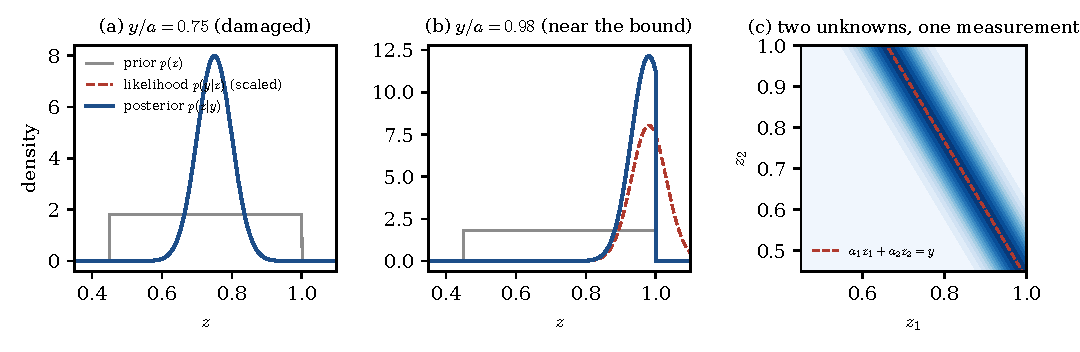
\includegraphics[width=\linewidth]{examples.pdf}
\caption{Worked examples, with $a=0.5$, $\sigma=0.025$, uniform prior on $[0.45,1]$. (a) Example~\ref{ex:1d} with $y/a=0.75$: the bounds are far from the likelihood peak, so the posterior coincides with the normalized likelihood (the dashed curve lies under the solid one). (b) The same with $y/a=0.98$: the bound $z=1$ cuts the likelihood, and the posterior is the truncated Gaussian. (c) Example~\ref{ex:2d}: one measurement of $0.5z_1+0.3z_2$; the posterior is a ridge along the line $a_1z_1+a_2z_2=y$, cut by the box.}
\label{fig:examples}
\end{figure}

\begin{example}[One unknown, one linear measurement, uniform prior]
\label{ex:1d}
Let a measurement depend linearly on one stiffness factor,
\begin{equation*}
y=a\,z+\varepsilon,\qquad\varepsilon\sim\N(0,\sigma^2),\qquad z\sim\U[\zlb,\zub],
\end{equation*}
with a sensitivity $a>0$ (e.g., $y$ is a log-frequency linearized around the healthy state, $a=\partial\log f/\partial z$).

\emph{Step 1: likelihood.} By Proposition~\ref{prop:likelihood}, $p(y|z)=p_\varepsilon(y-az)=\frac{1}{\sqrt{2\pi}\sigma}\exp\big(-\frac{(y-az)^2}{2\sigma^2}\big)$.

\emph{Step 2: write it as a function of $z$.} Factor $a$ out of the residual: $y-az=a\,(y/a-z)$, so $(y-az)^2=a^2(z-y/a)^2$, and
\begin{equation*}
\exp\Big(-\frac{(y-az)^2}{2\sigma^2}\Big)=\exp\Big(-\frac{a^2(z-y/a)^2}{2\sigma^2}\Big)=\exp\Big(-\frac{(z-\hat z)^2}{2s^2}\Big),\qquad \hat z=\frac ya,\quad s=\frac\sigma a.
\end{equation*}
As a function of $z$, the likelihood has the shape of a Gaussian centred at $\hat z$ with standard deviation $s$. (It is not a density in $z$; only its shape matters here.)

\emph{Step 3: multiply by the prior.} $p(z)=1/(\zub-\zlb)$ on $[\zlb,\zub]$ and zero outside, so
\begin{equation*}
p(z|y)\propto\exp\Big(-\frac{(z-\hat z)^2}{2s^2}\Big)\ind_{[\zlb,\zub]}(z).
\end{equation*}
All factors independent of $z$ ($1/(\sqrt{2\pi}\sigma)$, $1/(\zub-\zlb)$, $1/p(y)$) are absorbed in $\propto$.

\emph{Step 4: normalize.} With the substitution $\xi=(z-\hat z)/s$, $\dd z=s\dd\xi$:
\begin{equation*}
\int_{\zlb}^{\zub}\exp\Big(-\frac{(z-\hat z)^2}{2s^2}\Big)\dd z=s\int_{\alpha}^{\beta}e^{-\xi^2/2}\dd\xi=s\sqrt{2\pi}\,\big[\Psi(\beta)-\Psi(\alpha)\big],
\end{equation*}
with $\alpha=(\zlb-\hat z)/s$ and $\beta=(\zub-\hat z)/s$ (the limits of $\xi$), and $\int_\alpha^\beta e^{-\xi^2/2}\dd\xi=\sqrt{2\pi}\int_\alpha^\beta\varphi=\sqrt{2\pi}[\Psi(\beta)-\Psi(\alpha)]$.
Dividing by this integral,
\begin{equation*}
p(z|y)=\frac{\varphi\big((z-\hat z)/s\big)}{s\,\big[\Psi(\beta)-\Psi(\alpha)\big]},\qquad z\in[\zlb,\zub]:
\end{equation*}
a Gaussian with location $\hat z=y/a$ and scale $s=\sigma/a$, \emph{truncated} to the prior interval (Section~\ref{sec:tn}).

\emph{Interpretation.} $\hat z$ is the value of $z$ that reproduces the measurement exactly ($a\hat z=y$): the deterministic inverse. The scale $s=\sigma/a$ is the error divided by the sensitivity: a component to which the data are insensitive (small $a$) has a wide posterior.
With $\sigma=0.025$ (a $2.5\%$ frequency error in log scale, Example~\ref{ex:multiplicative}) and $a=0.5$, $s=0.05$.
If $\hat z$ is far from the bounds (more than about $3s$), $\Psi(\beta)-\Psi(\alpha)\approx1$ and the posterior is practically $\N(\hat z,s^2)$ (Fig.~\ref{fig:examples}a). If $\hat z$ is close to a bound, the posterior is cut and becomes asymmetric (Fig.~\ref{fig:examples}b): with $\hat z=0.98$, $\beta=(1-0.98)/0.05=0.4$, $\alpha=-10.6$, and the posterior mean, computed with Proposition~\ref{prop:tn_moments}, is $0.98-0.05\,\varphi(0.4)/\Psi(0.4)=0.98-0.05\times0.3683/0.6554=0.952$, lower than $\hat z$ because the values above 1 are excluded.
This is the situation of the healthy components, and the reason why truncated families are the natural choice for the marginals.
\end{example}

\begin{example}[One unknown, Gaussian prior: precisions add]
\label{ex:conjugate}
Replace the uniform prior by $z\sim\N(\mu_0,\tau^2)$ (no bounds). Then
\begin{equation*}
p(z|y)\propto\exp\Big(-\frac{(y-az)^2}{2\sigma^2}-\frac{(z-\mu_0)^2}{2\tau^2}\Big).
\end{equation*}
Expand the exponent and keep only the terms that depend on $z$:
\begin{equation*}
-\frac12\Big[\Big(\frac{a^2}{\sigma^2}+\frac1{\tau^2}\Big)z^2-2\Big(\frac{ay}{\sigma^2}+\frac{\mu_0}{\tau^2}\Big)z\Big]+\text{const}.
\end{equation*}
By Lemma~\ref{lem:square}(i) with $A=a^2/\sigma^2+1/\tau^2$ and $B=ay/\sigma^2+\mu_0/\tau^2$, the exponent is $-\frac A2(z-B/A)^2+\text{const}$, so the posterior is $\N(B/A,\,1/A)$:
\begin{equation*}
\frac{1}{\sigma_{\text{post}}^2}=\underbrace{\frac{a^2}{\sigma^2}}_{\text{data}}+\underbrace{\frac{1}{\tau^2}}_{\text{prior}},\qquad
\mu_{\text{post}}=\frac{\frac{a^2}{\sigma^2}\,\hat z+\frac1{\tau^2}\,\mu_0}{\frac{a^2}{\sigma^2}+\frac1{\tau^2}},\quad\hat z=\frac ya,
\end{equation*}
where we wrote $ay/\sigma^2=(a^2/\sigma^2)(y/a)$. The precisions (inverse variances) of the data and of the prior add, and the posterior mean is the precision-weighted average of the deterministic inverse and of the prior mean. For a very wide prior ($\tau\to\infty$) we recover Example~\ref{ex:1d} without bounds.
\end{example}

\begin{example}[Linear Gaussian inverse problem in $D$ dimensions]
\label{ex:linear_gauss}
Let $\m=\Ab\z+\eps$, $\eps\sim\N(\mathbf0,\Cb)$, and $\z\sim\N(\mub_0,\Sig_0)$. Then
\begin{equation*}
-\log p(\z|\m)=\tfrac12(\m-\Ab\z)^\top\Cb^{-1}(\m-\Ab\z)+\tfrac12(\z-\mub_0)^\top\Sig_0^{-1}(\z-\mub_0)+\text{const}.
\end{equation*}
Expand, using the symmetry of $\Cb^{-1}$ and $\Sig_0^{-1}$ (so that $\m^\top\Cb^{-1}\Ab\z=\z^\top\Ab^\top\Cb^{-1}\m$):
\begin{equation*}
-\log p(\z|\m)=\tfrac12\z^\top\big(\Ab^\top\Cb^{-1}\Ab+\Sig_0^{-1}\big)\z-\z^\top\big(\Ab^\top\Cb^{-1}\m+\Sig_0^{-1}\mub_0\big)+\text{const}.
\end{equation*}
By the consequence of Lemma~\ref{lem:square}(ii), the posterior is Gaussian with
\begin{equation*}
\Sig_{\text{post}}=\big(\Ab^\top\Cb^{-1}\Ab+\Sig_0^{-1}\big)^{-1},\qquad \mub_{\text{post}}=\Sig_{\text{post}}\big(\Ab^\top\Cb^{-1}\m+\Sig_0^{-1}\mub_0\big).
\end{equation*}
The matrix $\Ab^\top\Cb^{-1}\Ab$ is the information that the data carry on $\z$. If it is singular (fewer independent measurements than unknowns) or ill-conditioned (nearly dependent columns of $\Ab$: two unknowns with almost the same effect on the data), the data alone do not determine $\z$, and the prior decides in the uninformed directions. This is the probabilistic form of ill-posedness. A nonlinear forward model (our eigenvalue problem) behaves locally like this linear one, with $\Ab$ the Jacobian $\partial\Dc/\partial\z$, but the posterior is no longer exactly Gaussian.
\end{example}

\begin{example}[Two unknowns, one measurement: correlated posterior]
\label{ex:2d}
Let $y=a_1z_1+a_2z_2+\varepsilon$, $\varepsilon\sim\N(0,\sigma^2)$, with $a_1,a_2>0$; this is Example~\ref{ex:linear_gauss} with $\Ab=[a_1\ a_2]$. With a prior $\N(\mub_0,\tau^2\I)$, the posterior precision is
\begin{equation*}
\Pb=\frac1{\sigma^2}\begin{pmatrix}a_1^2&a_1a_2\\a_1a_2&a_2^2\end{pmatrix}+\frac1{\tau^2}\I.
\end{equation*}
The data part has determinant $a_1^2a_2^2-(a_1a_2)^2=0$: one measurement cannot determine two unknowns.
The inverse of a $2\times2$ matrix is $\Pb^{-1}=\frac1{\det\Pb}\begin{pmatrix}P_{22}&-P_{12}\\-P_{12}&P_{11}\end{pmatrix}$, so the posterior correlation is
\begin{equation*}
\rho_{12}=\frac{(\Pb^{-1})_{12}}{\sqrt{(\Pb^{-1})_{11}(\Pb^{-1})_{22}}}=\frac{-P_{12}}{\sqrt{P_{11}P_{22}}}
=-\frac{a_1a_2/\sigma^2}{\sqrt{\big(a_1^2/\sigma^2+1/\tau^2\big)\big(a_2^2/\sigma^2+1/\tau^2\big)}}\ \xrightarrow{\ \tau\to\infty\ }\ -1.
\end{equation*}
With a weak prior the two unknowns are almost perfectly negatively correlated: if $z_1$ is larger, $z_2$ must be smaller to explain the same $y$.
With the uniform prior (Fig.~\ref{fig:examples}c), the likelihood depends on $\z$ only through $a_1z_1+a_2z_2$: it is constant along the lines $a_1z_1+a_2z_2=\text{const}$, and, since the distance of a point $\z$ from the line $\aaa^\top\z=y$ is $|y-\aaa^\top\z|/\|\aaa\|$, it decays across the line as a Gaussian of standard deviation $\sigma/\|\aaa\|$:
\begin{equation*}
\exp\Big(-\frac{(y-\aaa^\top\z)^2}{2\sigma^2}\Big)=\exp\Big(-\frac{\text{dist}(\z)^2}{2(\sigma/\|\aaa\|)^2}\Big).
\end{equation*}
The posterior is a narrow ridge along the line, cut by the box: precise along one direction, uninformative along the other.
This is the situation of an end zone of the deck and the adjacent bearing, which have similar effects on the first modes. A posterior family with independent components cannot represent this ridge; the Gaussian copula can (Section~\ref{sec:copulas}).
\end{example}

% =====================================================================================================
\part{Variational inference}
\label{part:vi}

\section{Entropy and Kullback--Leibler divergence}
\label{sec:kl}

\subsection{Differential entropy}
\begin{definition}
The (differential) entropy of a density $q$ is
\begin{equation}
\Hent[q]=-\E_q[\log q(\z)]=-\int q(\z)\log q(\z)\dd\z.
\end{equation}
\end{definition}
It is the expectation of the function $-\log q(\z)$ when $\z$ is drawn from $q$ itself. It measures the spread of $q$: a density that spreads its mass over a large region takes small values there, so $-\log q$ is large.

\begin{example}[Uniform density]
On $[a,b]$, $q(z)=1/(b-a)$ for every $z$ in the interval. The function $-\log q(z)=-\log\frac1{b-a}=\log(b-a)$ is therefore a constant, and the expectation of a constant is the constant itself:
\begin{equation*}
\Hent[q]=\int_a^b q(z)\,\big(-\log q(z)\big)\dd z=\int_a^b\frac1{b-a}\log(b-a)\dd z=\log(b-a)\underbrace{\int_a^b\frac{\dd z}{b-a}}_{=1}=\log(b-a).
\end{equation*}
The entropy does not depend on $z$ (it is a number that characterizes the whole density); it depends on the length of the interval: the wider the interval, the larger the entropy. On the box $\Sset$, $q=1/(\zub-\zlb)^D$, and the same computation gives $\Hent=D\log(\zub-\zlb)$. With $\zub-\zlb=0.55<1$, this entropy is negative: differential entropy can be negative, because a density can exceed one.
\end{example}

\begin{example}[Gaussian density]
For $q=\N(\mu,\sigma^2)$, by \eqref{eq:gauss_pdf},
\begin{equation*}
-\log q(z)=\tfrac12\log(2\pi\sigma^2)+\frac{(z-\mu)^2}{2\sigma^2}.
\end{equation*}
Take the expectation under $q$. The first term is a constant; for the second, $\E_q[(z-\mu)^2]=\sigma^2$ (Section~\ref{sec:gauss}):
\begin{equation*}
\Hent[q]=\tfrac12\log(2\pi\sigma^2)+\frac{\sigma^2}{2\sigma^2}=\tfrac12\log(2\pi\sigma^2)+\tfrac12\log e=\log\big(\sqrt{2\pi e}\,\sigma\big).
\end{equation*}
The entropy grows with $\log\sigma$ and does not depend on $\mu$ (shifting a density does not change its spread). It is negative for $\sigma<1/\sqrt{2\pi e}\approx0.24$.
\end{example}

\begin{lemma}[Entropy under a change of variables]
\label{lem:entropy_cov}
Let $W$ have density $q_W$ and $Z=g(W)$ with $g$ strictly monotone and differentiable. Then $\Hent[Z]=\Hent[W]+\E\big[\log|g'(W)|\big]$.
\end{lemma}
\begin{proof}
By Proposition~\ref{prop:cov1d}, $q_Z(g(w))=q_W(w)/|g'(w)|$. Hence
\begin{equation*}
-\log q_Z(Z)=-\log q_W(W)+\log|g'(W)|,
\end{equation*}
and taking the expectation of both sides gives the result.
\end{proof}
Two uses: for the affine map $z=\zlb+(\zub-\zlb)x$, $g'=\zub-\zlb$ and $\Hent[z]=\Hent[x]+\log(\zub-\zlb)$; for $z=e^w$, $g'(w)=e^w$, $\log g'(w)=w$, and $\Hent[z]=\Hent[w]+\E[w]$ (Section~\ref{sec:logn}).

\subsection{The Kullback--Leibler divergence}
\begin{definition}
The Kullback--Leibler (KL) divergence of $q$ from $p$ is \cite{kullback1951,cover2006}
\begin{equation}
\KL(q\,\|\,p)=\E_q\Big[\log\frac{q(\z)}{p(\z)}\Big]=\int q(\z)\log\frac{q(\z)}{p(\z)}\dd\z.
\end{equation}
\end{definition}
It compares two densities by the average, under $q$, of the log-ratio of their values.

\begin{proposition}[Gibbs' inequality]
\label{prop:gibbs}
$\KL(q\,\|\,p)\ge0$, with equality if and only if $q=p$.
\end{proposition}
\begin{proof}
Apply Lemma~\ref{lem:log} with $t=p(\z)/q(\z)$ at every point where $q>0$:
\begin{equation*}
-\KL(q\,\|\,p)=\int_{q>0}q\log\frac pq\dd\z\le\int_{q>0}q\Big(\frac pq-1\Big)\dd\z=\int_{q>0}p\dd\z-\int_{q>0}q\dd\z\le1-1=0.
\end{equation*}
Equality requires $p/q=1$ wherever $q>0$ (equality in Lemma~\ref{lem:log}) and $\int_{q>0}p=1$, i.e., $p=q$.
\end{proof}
So the KL divergence behaves like a distance: it is zero only when the densities coincide. It is not symmetric, $\KL(q\,\|\,p)\neq\KL(p\,\|\,q)$ in general.

\paragraph{The support condition.} If $q>0$ on a region where $p=0$, then $\log(q/p)=+\infty$ there, and $\KL(q\,\|\,p)=\infty$. With the uniform prior, the posterior is zero outside $\Sset$. Therefore any approximate posterior with mass outside $\Sset$ is infinitely far from the posterior: an untruncated Gaussian marginal is not ``slightly wrong'', it is inadmissible.

\paragraph{KL from the uniform prior.} If $p$ is the uniform prior~\eqref{eq:prior} and $q$ is supported in $\Sset$, then $\log p(\z)=-D\log(\zub-\zlb)$ for every $\z$ where $q>0$, and
\begin{equation}
\KL(q\,\|\,p)=\E_q[\log q]-\E_q[\log p]=-\Hent[q]+D\log(\zub-\zlb).
\label{eq:kl_uniform}
\end{equation}
Being close to the uniform prior means having a large entropy.

\subsection{Reverse and forward KL}
\label{sec:reverse_kl}
Variational inference minimizes the \emph{reverse} divergence $\KL(q\,\|\,p)$, in which the average is taken under $q$.
Where $q>0$ but $p\approx0$, $\log(q/p)$ is very large: the reverse KL heavily penalizes putting mass where the target has none, and does not penalize ignoring regions where the target has mass (they do not contribute to the average under $q$). It is \emph{mode seeking}: a unimodal $q$ fitted to a bimodal $p$ locks onto one mode (Fig.~\ref{fig:tempering}b, blue).
The \emph{forward} divergence $\KL(p\,\|\,q)$, averaged under $p$, penalizes $q\approx0$ where $p>0$: it is \emph{mass covering}. For a Gaussian $q=\N(\mu,s^2)$, its minimizer has a simple form:
\begin{equation*}
\KL(p\,\|\,q)=-\Hent[p]-\E_p[\log q]=-\Hent[p]+\tfrac12\log(2\pi s^2)+\frac{\E_p[(z-\mu)^2]}{2s^2}.
\end{equation*}
Setting the derivative with respect to $\mu$ to zero gives $\E_p[z-\mu]=0$, i.e., $\mu=\E_p[z]$; setting the derivative with respect to $s$ to zero gives $1/s-\E_p[(z-\mu)^2]/s^3=0$, i.e., $s^2=\Var_p[z]$: the forward-KL Gaussian matches the mean and variance of $p$, and straddles both modes (Fig.~\ref{fig:tempering}b, red).
Consequence for the VAE: if the posterior is multimodal and the family is unimodal, the VAE tends to pick one mode and to underestimate the uncertainty, not to average the modes.

\begin{figure}[t]
\centering
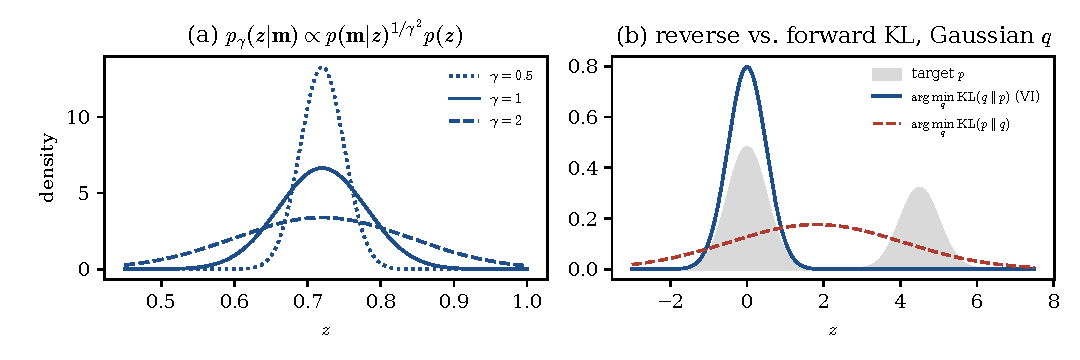
\includegraphics[width=\linewidth]{tempering_kl.pdf}
\caption{(a) Tempered posteriors $p_\gamma\propto p(\m|z)^{1/\gamma^2}p(z)$ for a Gaussian likelihood and a uniform prior on $[0.45,1]$ (Section~\ref{sec:tempering}). (b) Best Gaussian approximation of a bimodal density under the reverse KL (the VI objective, mode seeking; found by a grid search) and under the forward KL (mean and variance matched, mass covering).}
\label{fig:tempering}
\end{figure}

% -----------------------------------------------------------------------------------------------------
\section{Variational inference and the evidence lower bound}
\label{sec:vi}

\subsection{The variational problem}
Variational inference (VI) \cite{blei2017vi,zhang2019advances,bishop2006} chooses a family $\mathcal Q$ of tractable densities (easy to sample and to evaluate) and looks for the member closest to the posterior:
\begin{equation}
q^\star=\arg\min_{q\in\mathcal Q}\KL\big(q(\z)\,\|\,p(\z|\m)\big).
\label{eq:vi_problem}
\end{equation}
This objective cannot be evaluated directly: the posterior contains the evidence $p(\m)$, which is the intractable integral that we want to avoid. The ELBO removes it.

\subsection{Derivation of the ELBO}
\begin{proposition}[Evidence decomposition]
\label{prop:elbo}
For every density $q$ supported in $\Sset$ and every observation $\m$,
\begin{equation}
\log p(\m)=\ELBO(q;\m)+\KL\big(q\,\|\,p(\cdot|\m)\big),
\qquad
\ELBO(q;\m):=\E_q\big[\log p(\m,\z)-\log q(\z)\big].
\label{eq:evidence_decomposition}
\end{equation}
\end{proposition}
\begin{proof}
Write the KL divergence and replace the posterior using Bayes' theorem, $\log p(\z|\m)=\log p(\m,\z)-\log p(\m)$:
\begin{align*}
\KL\big(q\,\|\,p(\cdot|\m)\big)
&=\E_q\big[\log q(\z)-\log p(\z|\m)\big]\\
&=\E_q\big[\log q(\z)-\log p(\m,\z)+\log p(\m)\big]\\
&=\E_q\big[\log q(\z)-\log p(\m,\z)\big]+\log p(\m)\\
&=-\ELBO(q;\m)+\log p(\m),
\end{align*}
where $\log p(\m)$ was taken out of the expectation because it does not depend on $\z$ (and $\E_q[1]=1$).
\end{proof}

Since $\KL\ge0$ (Proposition~\ref{prop:gibbs}), $\ELBO(q;\m)\le\log p(\m)$: the ELBO is a \emph{lower bound} of the log-evidence. More importantly, $\log p(\m)$ does not depend on $q$, so increasing the ELBO by some amount decreases the KL divergence by exactly the same amount:
\begin{equation}
\boxed{\ \arg\max_{q\in\mathcal Q}\ELBO(q;\m)=\arg\min_{q\in\mathcal Q}\KL\big(q\,\|\,p(\cdot|\m)\big).\ }
\end{equation}
The ELBO contains only $p(\m,\z)=p(\m|\z)p(\z)$ (likelihood times prior, both computable) and $q$: maximizing it solves the variational problem without knowing $p(\m)$. If $\mathcal Q$ contains the posterior, the maximizer is the posterior itself.

\subsection{Three equivalent forms of the ELBO}
Expanding $\log p(\m,\z)=\log p(\m|\z)+\log p(\z)$ and using $\Hent[q]=-\E_q[\log q]$:
\begin{align}
\ELBO(q;\m)&=\underbrace{\E_q[\log p(\m|\z)]}_{\text{data fit}}+\underbrace{\E_q[\log p(\z)]}_{\text{prior}}+\underbrace{\Hent[q]}_{\text{entropy}}
\label{eq:elbo_a}\\
&=\E_q[\log p(\m|\z)]-\KL\big(q\,\|\,p(\z)\big)
\label{eq:elbo_b}\\
&=\log p(\m)-\KL\big(q\,\|\,p(\z|\m)\big).
\label{eq:elbo_c}
\end{align}
Form \eqref{eq:elbo_b} follows from \eqref{eq:elbo_a} because $\E_q[\log p(\z)]+\Hent[q]=\E_q[\log p(\z)-\log q(\z)]=-\KL(q\,\|\,p(\z))$; form \eqref{eq:elbo_c} is Proposition~\ref{prop:elbo}.
Reading of \eqref{eq:elbo_b}: the first term rewards densities whose samples reproduce the data (it alone would concentrate $q$ on the maximum-likelihood solutions); the second keeps $q$ close to the prior (a regularizer). Reading of \eqref{eq:elbo_a}: without the entropy, the best $q$ would be a point mass at the most likely $\z$ (a point estimate). The entropy is the only term that rewards uncertainty; its weight decides the width of the estimated posterior.

\subsection{The uniform-prior case: the loss used in the manuscripts}
With the uniform prior, $\E_q[\log p(\z)]=-D\log(\zub-\zlb)$ is a constant (Eq.~\eqref{eq:kl_uniform}), and the negative ELBO is
\begin{equation}
\boxed{\ -\ELBO(q;\m)=\E_q\big[\NLL(\z;\m)\big]-\Hent[q]+\text{const}
=\E_q\big[\NLL(\z;\m)\big]+\E_q\big[\log q(\z)\big]+\text{const}.\ }
\label{eq:neg_elbo_uniform}
\end{equation}
The term $\E_q[\log q]$ is the ``PDF term'' $\Lc_{\text{PDF}}$ of the manuscripts, the term ``$\log q_{\thetab}(\z^h|\m)$'' of the published copula paper \cite{fernandez2026pem}, and minus the entropy.
Everything that follows is a careful evaluation of~\eqref{eq:neg_elbo_uniform}: the NLL must be the negative log-density of the actual error model (Section~\ref{sec:likelihood}), $\log q$ must be the log-density of the distribution that generates the samples, and both terms must have weight one.

\subsection{The Gibbs variational principle}
The next lemma tells what \emph{any} loss of the form ``misfit $+$ weight $\times\,\E_q[\log q]$'' estimates.
\begin{lemma}[Gibbs variational principle]
\label{lem:gibbs_principle}
Let $a(\z)$ be a function with $C_a:=\int_{\Sset} e^{-a(\z)}\dd\z<\infty$, and $p_a(\z)=e^{-a(\z)}\ind_{\Sset}(\z)/C_a$. For every density $q$ supported in $\Sset$,
\begin{equation}
\E_q[a(\z)]-\Hent[q]=\KL(q\,\|\,p_a)-\log C_a.
\end{equation}
Hence the minimizer of $\E_q[a]-\Hent[q]$ over all densities is $p_a\propto e^{-a}$ on $\Sset$; over a family $\mathcal Q$, it is the member closest to $p_a$ in reverse KL.
\end{lemma}
\begin{proof}
$\log p_a(\z)=-a(\z)-\log C_a$ on $\Sset$, so $\KL(q\,\|\,p_a)=\E_q[\log q]-\E_q[\log p_a]=-\Hent[q]+\E_q[a]+\log C_a$. The minimizer follows from Proposition~\ref{prop:gibbs}, since $\log C_a$ does not depend on $q$.
\end{proof}
With $a=\NLL$ and the uniform prior, $p_a\propto p(\m|\z)\ind_{\Sset}$ is the posterior: this is Proposition~\ref{prop:elbo} again. Section~\ref{sec:tempering} applies the lemma to other weights.

% -----------------------------------------------------------------------------------------------------
\section{Amortized variational inference: the VAE}
\label{sec:amortized}

\subsection{From one observation to all observations}
Classical VI solves~\eqref{eq:vi_problem} separately for each observation, with its own parameters $\zetab$ of $q$ (e.g., a mean and a standard deviation per component). \emph{Amortized} VI \cite{kingma2014vae,rezende2014,zhang2019advances} learns a function, the encoder $\mathcal E_{\thetab}$ (a neural network with weights $\thetab$), that maps any observation to the parameters of its approximate posterior, $\zetab=\mathcal E_{\thetab}(\m)$; we write $\qth(\z|\m)$. The optimization is done once, during training; at inference, one forward pass of the encoder gives the posterior of a new observation.
The training loss is the negative ELBO averaged over the training observations:
\begin{equation}
\Lc(\thetab)=-\frac{1}{\Ntr}\sum_{i=1}^{\Ntr}\ELBO\big(\qth(\cdot|\m_i);\m_i\big).
\label{eq:amortized_loss}
\end{equation}

\begin{proposition}[What amortized training estimates]
\label{prop:amortized}
Let the training observations be draws from a distribution $p_{\text{data}}(\m)$. Then
\begin{equation}
\E_{p_{\text{data}}}\big[-\ELBO(\qth(\cdot|\m);\m)\big]=\E_{p_{\text{data}}}\Big[\KL\big(\qth(\cdot|\m)\,\|\,p(\cdot|\m)\big)\Big]-\E_{p_{\text{data}}}\big[\log p(\m)\big].
\end{equation}
The second term does not depend on $\thetab$. If the encoder can represent any map from observations to parameters, the minimizer gives, for every $\m$ in the support of $p_{\text{data}}$, the member of $\mathcal Q$ closest to the posterior defined by the likelihood and the prior of the loss.
\end{proposition}
\begin{proof}
Apply Proposition~\ref{prop:elbo} to each $\m$ and take the expectation. The first expectation is an average of non-negative terms, one per observation; if the encoder can choose the parameters of each observation independently, the average is minimized by minimizing each term.
\end{proof}

Three consequences:
\begin{enumerate}
\item \emph{The true damage condition never enters the loss.} The loss uses only the observations $\m_i$; the labels $\z^{\text{true}}_i$ of the training scenarios are not used. The VAE is not a regression of $\z$ on $\m$: it learns, for each $\m$, the distribution of the damage conditions compatible with $\m$.
\item \emph{The design of experiments weights, but does not bias.} The target of each $\m$ is the posterior defined by the prior in the loss (uniform), whatever the composition of the training set (Remark~\ref{rem:doe}). The composition decides where in the observation space the encoder is accurate, because the average KL weights each region by how often it appears in training.
\item \emph{Two gaps.} The estimate differs from the posterior because the family cannot represent it (approximation gap) or because the encoder does not reach the best member for every $\m$ (amortization gap) \cite{cremer2018}. The comparison with the SMC reference measures the sum of both.
\end{enumerate}

\subsection{Standard VAE versus physics-informed VAE}
In the standard VAE \cite{kingma2014vae}, the decoder $p_{\bm\psi}(\m|\z)$ is a neural network trained jointly with the encoder, the prior is $\N(\mathbf0,\I)$, and $\z$ has no physical meaning. In our VAE, the decoder is the FE model with the eigenvalue solver (no trainable parameters), $\z$ is the vector of physical stiffness factors, the likelihood is fixed by the error model, the prior is the uniform box, and only the encoder is trained. The method is amortized Bayesian inference with a known physical likelihood. The published copula paper \cite{fernandez2026pem} uses a pretrained neural surrogate of the forward model, frozen while the encoder is trained: the reasoning is the same.

% -----------------------------------------------------------------------------------------------------
\section{Gradients: Monte Carlo and the reparameterization trick}
\label{sec:reparam}

\subsection{The problem}
The loss contains $\E_{\qth}[\NLL(\z;\m)]$, an expectation under a density that depends on $\thetab$. It has no closed form (each NLL needs an eigenvalue analysis), so it is estimated by Monte Carlo (Proposition~\ref{prop:mc}) with samples $\z^h\sim\qth$. Gradient descent needs the derivative of this estimate with respect to $\thetab$, but ``a sample drawn from $\qth$'' is not, as such, a function of $\thetab$ that can be differentiated.

\subsection{The reparameterization (pathwise) gradient}
The trick \cite{kingma2014vae,rezende2014,mohamed2020mcgrad} writes the sample as a differentiable transformation of a noise whose distribution does not depend on $\thetab$:
\begin{equation}
\z=T_{\thetab}(\eps),\qquad\eps\sim p(\eps)\ \text{(fixed)}.
\end{equation}
Then $\E_{\qth}[g(\z)]=\E_{p(\eps)}[g(T_{\thetab}(\eps))]=\int g(T_{\thetab}(\eps))\,p(\eps)\dd\eps$. Now $\thetab$ appears only inside the integrand, and the density $p(\eps)$ does not depend on it, so, for smooth integrands, the derivative can be taken inside the integral (chain rule on $g\circ T_{\thetab}$):
\begin{equation}
\nabla_{\thetab}\E_{\qth}[g(\z)]=\E_{p(\eps)}\Big[\nabla_{\z}g\big(T_{\thetab}(\eps)\big)\,\frac{\partial T_{\thetab}(\eps)}{\partial\thetab}\Big]
\approx\frac1H\sum_{h=1}^H\nabla_{\z}g(\z^h)\,\frac{\partial T_{\thetab}(\eps^h)}{\partial\thetab}.
\end{equation}
The approximation is a Monte Carlo average, unbiased by Proposition~\ref{prop:mc}.

\begin{example}[A check]
Let $z\sim\N(\mu,\sigma^2)$ and $g(z)=z^2$. Directly, $\E[z^2]=\Var[z]+\E[z]^2=\sigma^2+\mu^2$, whose derivative with respect to $\mu$ is $2\mu$. With $z=T(\varepsilon)=\mu+\sigma\varepsilon$, $\varepsilon\sim\N(0,1)$: $\partial T/\partial\mu=1$ and $g'(z)=2z$, so the pathwise gradient is $\E[2(\mu+\sigma\varepsilon)]=2\mu$. The two agree.
\end{example}

In our VAE, $g=\NLL$: $\nabla_{\z}\NLL$ requires the derivatives of the eigenvalues and eigenvectors with respect to the stiffness factors, which automatic differentiation of the symmetric eigensolver provides; $\partial T/\partial\thetab$ is the derivative of the sampler. Examples of $T_{\thetab}$:
\begin{itemize}
\item Gaussian: $z=\mu+\sigma\varepsilon$, $\varepsilon\sim\N(0,1)$ (Section~\ref{sec:gauss}).
\item Gaussian vector: $\y=\Lb\eps$, $\eps\sim\N(\mathbf0,\I)$, has distribution $\N(\mathbf0,\Lb\Lb^\top)$ (Proposition~\ref{prop:mvn}).
\item Any continuous distribution on $\R$: $z=F^{-1}(u;\thetab)$, $u\sim\U(0,1)$ (Lemma~\ref{lem:pit}).
\item The Gaussian copula: a composition of the previous two (Algorithm~\ref{alg:copula_sampling}).
\end{itemize}

\paragraph{The alternative: the score-function estimator.} Differentiating $\int g(\z)\qth(\z)\dd\z$ directly gives $\int g\,\nabla_{\thetab}\qth\dd\z=\E_{\qth}[g\,\nabla_{\thetab}\log\qth]$, using $\nabla q=q\nabla\log q$. It needs no derivative of $g$ (useful for discrete variables), but its variance is typically much larger, because it uses only the values of $g$, not its slope. The pathwise estimator is the standard choice when $g$ is differentiable.

\subsection{Gradient through an inverse CDF}
\label{sec:implicit}
When $F^{-1}$ has a closed form (truncated Gaussian, truncated log-normal, Kumaraswamy), $\partial z/\partial\thetab$ is obtained by differentiating the formula. When it does not (mixtures), $z$ is computed numerically (bisection, Newton), and the derivative of a numerical loop is not available. It is obtained by \emph{implicit differentiation} \cite{figurnov2018implicit}: $z(\thetab)$ is defined by the identity $F(z(\thetab);\thetab)=u$ at fixed $u$; differentiating both sides with respect to $\thetab$ (chain rule; the right-hand side is constant):
\begin{equation}
\underbrace{\frac{\partial F}{\partial z}}_{=q(z;\thetab)}\frac{\partial z}{\partial\thetab}+\frac{\partial F(z;\thetab)}{\partial\thetab}=0
\qquad\Longrightarrow\qquad
\boxed{\ \frac{\partial z}{\partial\thetab}=-\frac{\partial_{\thetab}F(z;\thetab)}{q(z;\thetab)}.\ }
\label{eq:implicit_grad}
\end{equation}
Only the CDF and the density are needed, not the root-finding algorithm. Interpretation: if a change of $\thetab$ increases $F$ at $z$ (more mass below $z$), the quantile of level $u$ must move to the left, and it moves less where the density is large.

\subsection{Entropy: closed form or Monte Carlo}
The entropy term can be estimated by Monte Carlo, $\Hent[\qth]\approx-\frac1H\sum_h\log\qth(\z^h)$ with $\z^h=T_{\thetab}(\eps^h)$, or computed in closed form when available. The closed form removes one source of noise from the gradient and is used whenever possible (Section~\ref{sec:copula_entropy}). In the Monte Carlo estimate, $\log\qth(T_{\thetab}(\eps);\thetab)$ depends on $\thetab$ through the sample and through the density. The second dependence (the score $\nabla_{\thetab}\log\qth$ at fixed $\z$) has zero mean, because $\E_q[\nabla_{\thetab}\log q]=\int\nabla_{\thetab}q\dd\z=\nabla_{\thetab}\int q\dd\z=\nabla_{\thetab}1=0$; it only adds noise and can be dropped \cite{roeder2017sticking}.

\subsection{Why rejection sampling and clipping are problematic}
\label{sec:rejection}
To keep the samples inside $\Sset$, one can (a) draw from an untruncated density $q$ and reject the samples outside $\Sset$, or (b) clip them to the bounds.

\emph{Rejection.} Let $C(\thetab)=\int_{\Sset} q\dd\z$ be the probability that a proposal is accepted. The accepted samples have density $\tilde q=q\,\ind_{\Sset}/C(\thetab)$: for any set $A$, $P(\z\in A\,|\,\text{accepted})=P(\z\in A\cap\Sset)/P(\z\in\Sset)=\int_{A\cap\Sset}q\dd\z/C(\thetab)$. Two consequences:
\begin{itemize}
\item the log-density in the loss must be $\log\tilde q=\log q-\log C(\thetab)$; if $C$ is omitted, the entropy is wrong, and so is its gradient, because $C$ depends on $\thetab$;
\item the accepted sample is not a smooth function of $\thetab$: when $\thetab$ changes, a proposal can cross the boundary of $\Sset$, and then a different proposal is accepted (a jump). The pathwise derivative of the accepted sample ignores these jumps, so it misses part of the gradient of the expectation.
\end{itemize}
The cost also grows when much mass lies outside $\Sset$, which is precisely the case of healthy components, whose mass is piled against $z=1$.

\emph{Clipping} moves all the mass outside $\Sset$ onto the bounds: the clipped variable equals $\zub$ with positive probability (an atom), it has no density there, and its entropy is $-\infty$.

Inverse-CDF sampling of a truncated family has none of these problems: every sample is valid, its density is known exactly, and the transformation is smooth.

% -----------------------------------------------------------------------------------------------------
\section{Temperature, $\gamma$, and warm-up}
\label{sec:tempering}

\subsection{The tempered posterior}
Both manuscripts weight the entropy term by $\gamma^2$:
\begin{equation}
\Lc_\gamma(q;\m)=\E_q[\NLL(\z;\m)]-\gamma^2\Hent[q]=\E_q[\NLL(\z;\m)]+\gamma^2\E_q[\log q].
\label{eq:loss_gamma}
\end{equation}
\begin{proposition}
\label{prop:tempered}
The minimizer of~\eqref{eq:loss_gamma} over $\mathcal Q$ is the member closest in reverse KL to the tempered posterior
\begin{equation}
p_\gamma(\z|\m)\propto p(\m|\z)^{1/\gamma^2}\,\ind_{\Sset}(\z).
\end{equation}
\end{proposition}
\begin{proof}
Dividing a function by a positive constant does not change where its minimum is: minimize $\Lc_\gamma/\gamma^2=\E_q[\NLL/\gamma^2]-\Hent[q]$. Apply Lemma~\ref{lem:gibbs_principle} with $a=\NLL/\gamma^2$: $p_a\propto e^{-\NLL/\gamma^2}\ind_{\Sset}=\big(e^{-\NLL}\big)^{1/\gamma^2}\ind_{\Sset}\propto p(\m|\z)^{1/\gamma^2}\ind_{\Sset}$.
\end{proof}
For a Gaussian error model, $\NLL=\sum_jr_j^2/(2\sigma_j^2)$, and
\begin{equation*}
\exp\Big(-\frac{r_j^2}{2\sigma_j^2}\Big)^{1/\gamma^2}=\exp\Big(-\frac{r_j^2}{2\gamma^2\sigma_j^2}\Big)=\exp\Big(-\frac{r_j^2}{2(\gamma\sigma_j)^2}\Big):
\end{equation*}
\emph{the temperature $\gamma$ multiplies every error standard deviation by $\gamma$.} Hence (Fig.~\ref{fig:tempering}a): $\gamma=1$ gives the Bayesian posterior; $\gamma<1$ a narrower posterior (overconfident intervals, as if the data were more accurate than they are); $\gamma>1$ a wider one (conservative intervals). In Example~\ref{ex:1d}, the posterior scale becomes $\gamma\sigma/a$. This is the content of the appendix on $\gamma$ in the revised manuscript. In the machine learning literature the same weight appears as $\beta$ in the $\beta$-VAE \cite{higgins2017beta} ($\beta=\gamma^2$), and tempered posteriors are studied in generalized Bayesian inference \cite{bissiri2016general}. In the published copula paper \cite{fernandez2026pem}, instead, $\beta$ is the standard deviation of the error in $\Gamma=\mathrm{diag}(\beta^2)$, and the entropy weight is one.

\paragraph{The key point.} A loss ``misfit $+\,\gamma^2\E[\log q]$'' estimates the Bayesian posterior only if the misfit \emph{is} the NLL of the actual error model \emph{and} $\gamma=1$. Otherwise it still has a minimizer, but it is the tempered posterior of an error model with standard deviations $\gamma\sigma_j^{\text{implied}}$, where $\sigma_j^{\text{implied}}$ are those of the error model implied by the misfit (Remark~\ref{rem:misfit}).

\subsection{Warm-up (likelihood tempering)}
In the revised code, the first epochs use
\begin{equation}
\Lc_\tau=\tau\,\E_q[\NLL]-\gamma^2\Hent[q],\qquad \tau=\tau_0^{\,1-\text{epoch}/E_w}\ \text{for epoch}<E_w,\qquad\tau=1\ \text{afterwards},
\end{equation}
with $\tau_0=0.01$ and $E_w$ warm-up epochs (150 by default in the code). By Lemma~\ref{lem:gibbs_principle} with $a=\tau\NLL$ (and $\gamma=1$), the target during the warm-up is $p(\m|\z)^\tau\ind_{\Sset}$: with $\tau=0.01$ it is very close to the prior (broad posteriors), and it becomes the posterior when $\tau=1$. Starting broad avoids a common failure at the start of the training: with a random encoder, the steep likelihood term pushes $q$ to collapse onto a wrong point before the entropy can act. The warm-up changes only the path of the optimization, not its end point. The model is selected with the validation negative ELBO at $\tau=1$, after the warm-up.

% =====================================================================================================
\part{From the original loss function to the revised one}
\label{part:loss}

\section{The original formulation}
\label{sec:original}

\subsection{As written in the published copula-VAE paper}
The published paper \cite{fernandez2026pem} (its Section~3) derives the ELBO with the evidence decomposition of Proposition~\ref{prop:elbo} (its Eqs.~(14)--(16)), approximates the expectations with $H$ samples (its Eq.~(17)), assumes a Gaussian error $\N(\mathbf0,\Gamma)$ with $\Gamma=\mathrm{diag}(\beta^2)$ (its Eq.~(18)), drops the constant log-prior of the uniform prior, and trains with (its Eq.~(32))
\begin{equation}
\Lc_{\ELBO}(\thetab)\approx\frac{1}{\Ntr H}\sum_{i=1}^{\Ntr}\sum_{h=1}^{H}\Big[\tfrac12\big(\m_i-\mathcal F(\z_i^h,\mathbf w_i)\big)^\top\Gamma^{-1}\big(\m_i-\mathcal F(\z_i^h,\mathbf w_i)\big)+\log\qth(\z_i^h|\m_i,\mathbf w_i)\Big],
\label{eq:pem_loss}
\end{equation}
with $\beta=0.075$ in the MinMax-scaled units of the features, chosen empirically from prior work.

\paragraph{Is this a correct negative ELBO?} Yes in structure: it is~\eqref{eq:neg_elbo_uniform} with the NLL of Example~\ref{ex:corr_gauss} (factor $\tfrac12$, inverse covariance) and weight one on $\E[\log q]$. It estimates the Bayesian posterior if three conditions hold:
\begin{description}
\item[(C1)] $\Gamma$ is the covariance of the actual error of the scaled features (noise and modeling error, including the error of the surrogate decoder). If the true standard deviation is $\sigma$ and $\beta\neq\sigma$, the result is the tempered posterior with $\gamma=\beta/\sigma$ (Proposition~\ref{prop:tempered}).
\item[(C2)] $\log\qth$ is the log-density of the distribution that actually produced the samples, including the normalizer of any truncation (Section~\ref{sec:rejection}).
\item[(C3)] The prior is the uniform prior on the box, and $\qth$ is supported in the box (Section~\ref{sec:kl}).
\end{description}

\subsection{As implemented for the submitted CPENG-8674 manuscript}
The submitted manuscript writes $\Lc_{\ELBO}\approx\Lc_{\text{freq}}+\lambda\Lc_{\text{MAC}}+\gamma^2\Lc_{\text{PDF}}$ with $\lambda=10$ and $\gamma=0.30$. The code used for the runs of March 2026 (\texttt{MODULES/COPULAS/GC\_GMm\_models.py}, function \texttt{ELBO\_Copula\_loss}) computes, per observation and with $H=1$ sample,
\begin{equation}
\begin{aligned}
\Lc^{\text{orig}}={}&
\underbrace{\frac1{n_m}\sum_{j=1}^{n_m}\Big(\frac{\log f_j-\log\hat f_j}{s_j}\Big)^2}_{\text{frequencies}}
+\lambda\underbrace{\frac1{n_m}\sum_{j=1}^{n_m}\Big[\big(1-\MAC^{\text{best}}_{\text{v},j}\big)+\big(1-\MAC^{\text{best}}_{\text{r},j}\big)\Big]}_{\text{mode shapes (vertical and rotational)}}\\
&+\gamma^2\,\underbrace{\log\qth(\z|\m)}_{\log c+\sum_d\log q_d},
\end{aligned}
\label{eq:orig_loss}
\end{equation}
averaged over the mini-batch, where:
\begin{itemize}
\item $s_j$ is the standard deviation of $\log f_j$ \emph{over the training set} (the code standardizes the measured and the predicted log-frequencies with the same mean and $s_j$, and the mean cancels in the difference); $s_j$ measures how much $\log f_j$ varies among the scenarios, not how large its error is. The formula of the submitted manuscript does not show $s_j$;
\item the frequency term is a \emph{mean} over the modes, without the factor $\tfrac12$;
\item $\MAC^{\text{best}}_j=\max_k\MAC(\bm\phi_j,\hat{\bm\phi}_k)$ matches each measured mode with the best predicted mode, not with the predicted mode of the same order;
\item the samples come from the Gaussian copula with truncated Gaussian marginals: the copula uniforms $\uu$ are drawn by rejection, keeping only vectors with all $u_d\in(10^{-5},0.99)$, and then $z_d=F_d^{-1}(u_d)$;
\item $\log q$ is a one-sample Monte Carlo estimate of $\E[\log q]$, with the truncated-Gaussian log-density on $[\zlb-10^{-4},\,1+10^{-4}]$.
\end{itemize}
(Later versions of the code replaced the frequency MSE by a Huber loss and used $\lambda=15$; the analysis below is the same.)

\subsection{Which posterior did the original loss estimate?}
\label{sec:implied}
Dividing~\eqref{eq:orig_loss} by $\gamma^2$ does not change its minimizer. Rewrite each coefficient in the form of a Gaussian NLL with weight one on $\log q$:
\begin{equation*}
\frac{1}{\gamma^2}\cdot\frac{1}{n_m}\cdot\frac{(\log f_j-\log\hat f_j)^2}{s_j^2}=\frac{(\log f_j-\log\hat f_j)^2}{2\big(\sigma^{\text{eff}}_{f,j}\big)^2}
\quad\text{with}\quad 2\big(\sigma^{\text{eff}}_{f,j}\big)^2=\gamma^2n_ms_j^2,
\end{equation*}
\begin{equation*}
\frac{1}{\gamma^2}\cdot\frac{\lambda}{n_m}\,(1-\MAC_j)=\frac{1-\MAC_j}{2\big(\sigma^{\text{eff}}_{\Phi}\big)^2}
\quad\text{with}\quad 2\big(\sigma^{\text{eff}}_{\Phi}\big)^2=\frac{\gamma^2n_m}{\lambda}.
\end{equation*}
Hence the original loss is exactly the negative ELBO (with $\gamma=1$) of the error model with standard deviations
\begin{equation}
\sigma^{\text{eff}}_{f,j}=\gamma\,s_j\sqrt{\frac{n_m}{2}},\qquad
\sigma^{\text{eff}}_{\Phi}=\gamma\sqrt{\frac{n_m}{2\lambda}},
\label{eq:implied_sigma}
\end{equation}
where $(1-\MAC)/(2\sigma^2)$ is the Gaussian NLL of a mode shape with per-component error $\sigma$ (Section~\ref{sec:mac}).
Numbers for the submitted case study ($\gamma=0.30$, $n_m=5$, $\lambda=10$; 5 elements, noise $2.5\%$ on the frequencies and $5\%$ of the peak amplitude on the mode shapes; training data in \texttt{Data\_archive\_original\_paper/01Mar2026\_Noisy\_E5\_level25}, where $s_j=0.0504$--$0.0594$):
\begin{itemize}
\item \emph{Frequencies:} $\gamma\sqrt{n_m/2}=0.30\times\sqrt{2.5}=0.30\times1.581=0.474$, so $\sigma^{\text{eff}}_{f,j}=0.474\,s_j=0.024$--$0.028$. The true error of $\log f$ is $0.025$ (Example~\ref{ex:multiplicative}). The value $\gamma=0.30$, selected by the sensitivity study, happened to compensate the arbitrary standardization of the frequencies.
\item \emph{Mode shapes:} $\sigma^{\text{eff}}_\Phi=0.30\times\sqrt{5/20}=0.30\times0.5=0.15$. The true per-component error of a unit-norm shape is $s=0.05\times\max_k|v_k|$ (Section~\ref{sec:mac}); the mean peak component of the unit-norm vertical shapes of that data set is $0.616$--$0.701$, so $s=0.031$--$0.035$. The implied variance is $0.15^2/s^2=0.0225/0.00123$ to $0.0225/0.00095$, i.e., about 18--24 times the true one: the information of the mode shapes was down-weighted by a factor of about 20.
\end{itemize}
In short, the original loss is a negative ELBO in structure, but its ``likelihood'' was a discrepancy measure with weights chosen for numerical balance, and the width of the estimated posterior was set by the tuned value of $\gamma$, not by the error of the data.

\subsection{Why it did not estimate the Bayesian posterior: summary}
\begin{description}
\item[(P1) The misfit was not the likelihood of the error.] Standardization by the spread of the data set, averages over modes instead of sums, no factor $\tfrac12$ and the empirical weight $\lambda$ made the implied error model~\eqref{eq:implied_sigma} unrelated to the actual errors; frequencies and mode shapes were weighted inconsistently with their accuracy.
\item[(P2) $\gamma$ was a tuned temperature.] By Proposition~\ref{prop:tempered}, $\gamma$ rescales all error standard deviations; selecting it by performance metrics makes the posterior width a tuned hyperparameter. Moreover, the selection used metrics affected by an array-broadcasting error (MSE, MAE, coverage).
\item[(P3) Best-match MAC.] $\max_k\MAC(\bm\phi_j,\hat{\bm\phi}_k)$ lets a predicted mode be matched with a measured mode of a different order; that is not the likelihood of ordered modes. The revised loss compares modes of the same order; the sign is irrelevant because the MAC does not depend on it.
\item[(P4) Truncated copula sampling.] Rejecting $\uu\notin(10^{-5},0.99)^D$ removes the top $1\%$ of every marginal, i.e., the values closest to $z=1$, where the healthy components lie, and the density in $\log q$ was not renormalized (Section~\ref{sec:rejection}): the samples and the density of the loss did not match.
\item[(P5) Monte Carlo entropy with one sample.] Unbiased but noisy; the entropy of the Gaussian copula with truncated Gaussian or log-normal marginals has a closed form (Section~\ref{sec:copula_entropy}).
\item[(P6) No modeling error.] Not an issue in the submitted case study, where the data were generated with the decoder's own FE model; it becomes one in the revised case study (finer mesh, mass perturbation), where it is of the order of the noise and must be part of the error model.
\end{description}

\begin{remark}[Pitfalls of the Kumaraswamy-mixture prototype]
At the start of the revision, the prototype with Kumaraswamy-mixture marginals had additional issues (documented in \texttt{review29oct\_fixed/README.md}, Section~1.1), which show how fragile the balance of the terms is:
(i) the entropy entered with the wrong sign ($+\gamma^2\Hent$ instead of $-\gamma^2\Hent$), so the training \emph{minimized} the entropy and the copula became singular (correlations $\approx\pm1$), the only brake being a clip of $\log q$;
(ii) a boundary penalty $-\log x-\log(1-x)$ pushed the samples away from $z=1$, biasing every healthy component downwards;
(iii) the misfit was $5\times$Huber$+\,10\times(1-\MAC)$, again not the likelihood of the error;
(iv) clipping of the quantile gradients, and a learning rate that had decayed by a factor of $10^{-4}$ after about 1,900 epochs, effectively stopped the training.
With the correct sign of the entropy there is no incentive to collapse, and none of these devices is needed.
\end{remark}

% -----------------------------------------------------------------------------------------------------
\section{Derivation of the revised loss function}
\label{sec:revised}
The revised loss is~\eqref{eq:neg_elbo_uniform} evaluated with care: (i) the likelihood of an error model calibrated before training, (ii) the uniform prior, (iii) the exact entropy of the copula posterior, (iv) $\gamma=1$.

\subsection{Error model of the frequencies}
\label{sec:freq_error}
The data are simulated with multiplicative noise on the frequencies, $f^{\text{obs}}_j=f^{\text{true}}_j(1+\epsilon_j)$, $\epsilon_j\sim\N(0,\sigma_{\text{noise}}^2)$ independent, $\sigma_{\text{noise}}=0.025$. By Example~\ref{ex:multiplicative}, $\log f^{\text{obs}}_j=\log f^{\text{true}}_j+\eta_j$ with $\eta_j\approx\N(0,\sigma_{\text{noise}}^2)$.
The true structure (50 elements, perturbed masses) differs from the decoder (nominal FE model). Define the modeling error $\delta_j=\log f^{\text{true}}_j-\log\hat f_j(\z^{\text{true}})$. Then
\begin{equation*}
\log\mathbf f^{\text{obs}}=\log\hat{\mathbf f}(\z^{\text{true}})+\bm\delta+\bm\eta.
\end{equation*}
We model $\bm\delta\sim\N(\bb,\Cb_{\text{model}})$ (an assumption; $\bb$ captures a systematic offset, e.g., of the coarser mesh, and $\Cb_{\text{model}}$ is not diagonal, because a mass deviation shifts several frequencies together), independent of the noise. By Section~\ref{sec:combine},
\begin{equation}
\bm\delta+\bm\eta\sim\N\big(\bb,\ \Cb_f\big),\qquad \Cb_f=\Cb_{\text{model}}+\sigma_{\text{noise}}^2\I,
\end{equation}
and by Proposition~\ref{prop:likelihood} and Example~\ref{ex:corr_gauss}
\begin{equation}
\NLL_f(\z;\m)=\tfrac12\,\rr^\top\Cb_f^{-1}\rr+\text{const},\qquad \rr=\log\mathbf f^{\text{obs}}-\bb-\log\hat{\mathbf f}(\z).
\end{equation}
\paragraph{Calibration.} $\bb$ and $\Cb_{\text{model}}$ are estimated before training by simulation: 6,000 additional structures from the design of experiments, with new random mass fields, are computed with the true model and with the decoder for the same $\z$; $\bb$ is the sample mean and $\Cb_{\text{model}}$ the sample covariance of $\log f^{\text{true}}-\log\hat f$. These simulations are not part of the training, validation or test data. With a diagonal covariance, $\NLL_f=\sum_jr_j^2/(2\sigma_{f,j}^2)$, which is the form written in the revised manuscript; the code uses the full covariance and the offset $\bb$.

\subsection{Error model of the mode shapes and the MAC}
\label{sec:mac}
A mode shape is defined up to its scale and its sign: $\bm\phi$, $2\bm\phi$ and $-\bm\phi$ are the same mode. Only its \emph{direction} carries information, so the likelihood must depend only on the direction.

\paragraph{Noise model.} In the data, each component of each identified mode receives an independent Gaussian error with standard deviation equal to $5\%$ of the largest absolute component of that mode. If the shape is rescaled by any factor $c>0$, the error is rescaled by the same factor; so, for the unit-norm shape $\vv$ ($\|\vv\|=1$), the error of each component has standard deviation $s=0.05\max_k|v_k|$. The measured shape is, up to scale and sign, $\tilde\vv=\vv+\e$, with $\e\sim\N(\mathbf0,s^2\I_{n_s})$.

\paragraph{Geometry.} Decompose the error into its components along $\vv$ and perpendicular to $\vv$: $\e=(\vv^\top\e)\,\vv+\e_\perp$, with $\vv^\top\e_\perp=0$. The MAC of two vectors is the squared cosine of their angle:
\begin{equation}
\MAC(\tilde\vv,\vv)=\frac{(\vv^\top\tilde\vv)^2}{\|\vv\|^2\|\tilde\vv\|^2}.
\end{equation}
Here $\vv^\top\tilde\vv=1+\vv^\top\e$ and, by Pythagoras (the two parts are orthogonal), $\|\tilde\vv\|^2=(1+\vv^\top\e)^2+\|\e_\perp\|^2$. Hence
\begin{equation}
1-\MAC(\tilde\vv,\vv)=\frac{\|\e_\perp\|^2}{(1+\vv^\top\e)^2+\|\e_\perp\|^2}=\|\e_\perp\|^2\big(1+O(\|\e\|)\big),
\end{equation}
where the last step uses that $\vv^\top\e$ and $\|\e_\perp\|^2$ are small (of order $s$ and $s^2$) when the noise is small.

\paragraph{Likelihood.} The parallel component $\vv^\top\e$ only changes the length of $\tilde\vv$, which carries no information; the direction of $\tilde\vv$ is changed only by $\e_\perp$. The perpendicular part is $\e_\perp=\Pb_\perp\e$ with the projector $\Pb_\perp=\I-\vv\vv^\top$. In an orthonormal basis whose first vector is $\vv$ (Section~\ref{sec:linalg}(vi)), the coordinates of $\e$ are again independent $\N(0,s^2)$ (Lemma~\ref{lem:rotation}, scaled by $s$), and $\e_\perp$ consists of the last $n_s-1$ of them. So $\e_\perp$ has the Gaussian density $\propto\exp(-\|\e_\perp\|^2/(2s^2))$ in the $(n_s-1)$-dimensional subspace orthogonal to $\vv$, and, to leading order in the noise,
\begin{equation}
-\log p\big(\text{direction of }\tilde\vv\,\big|\,\z\big)=\frac{\|\e_\perp\|^2}{2s^2}+\text{const}\approx\frac{1-\MAC\big(\tilde\vv,\vv(\z)\big)}{2s^2}+\text{const}.
\end{equation}
The MAC is invariant to the sign and to the scale of either vector, so this likelihood does not depend on the arbitrary sign or normalization of the identified modes.

\paragraph{Expected value.} $\E\|\e_\perp\|^2=\E[\e^\top\Pb_\perp\e]=\tr(\Pb_\perp s^2\I)=s^2(n_s-1)$ (Lemma~\ref{lem:quadform} with $\mub=\mathbf0$; $\tr\Pb_\perp=\tr\I-\tr(\vv\vv^\top)=n_s-\vv^\top\vv=n_s-1$). Hence $\E[1-\MAC]\approx(n_s-1)s^2$. This identity is used to calibrate the modeling-error part of $s$ from simulations.

\paragraph{Total.} Adding the modeling error of the shapes (independent of the noise, so the variances add), the variance of mode $j$ is $\sigma_{\Phi,j}^2=s_{\text{noise},j}^2+s_{\text{model},j}^2$, and
\begin{equation}
\NLL_\Phi(\z;\m)=\sum_{j=1}^{n_m}\frac{1-\MAC_j\big(\bm\Phi,\hat{\bm\Phi}(\z)\big)}{2\,\sigma_{\Phi,j}^2},
\end{equation}
where $\MAC_j$ compares the $j$-th measured mode with the $j$-th predicted mode.

\subsection{The likelihood}
Assuming the errors of the frequencies and of the shapes independent (so that their densities multiply and their NLLs add),
\begin{equation}
\boxed{\ \NLL(\z;\m)=\tfrac12\,\rr^\top\Cb_f^{-1}\rr+\sum_{j=1}^{n_m}\frac{1-\MAC_j\big(\bm\Phi,\hat{\bm\Phi}(\z)\big)}{2\,\sigma_{\Phi,j}^2}.\ }
\label{eq:nll_revised}
\end{equation}
Every weight comes from the error model; there is no free weight such as $\lambda$. The calibration can be checked on simulated data: at the true $\z$, the expected value of each term is fixed by the error model ($\E[\tfrac12\rr^\top\Cb_f^{-1}\rr]=\tfrac12\tr(\Cb_f^{-1}\Cb_f)=\tfrac{n_m}2$ by Lemma~\ref{lem:quadform}, and $\E[(1-\MAC_j)/(2\sigma_{\Phi,j}^2)]\approx\tfrac{n_s-1}2$ by the previous section). The same function is used to train the VAE and to compute the SMC reference posterior, so both target the same posterior.

\subsection{Entropy of the copula posterior}
\label{sec:copula_entropy}
The posterior family is the Gaussian copula (Section~\ref{sec:copulas}),
\begin{equation}
\qth(\z|\m)=c_{\Sig}\big(F_1(z_1),\dots,F_D(z_D)\big)\prod_{d=1}^Dq_d(z_d),
\end{equation}
with the Gaussian copula density $c_{\Sig}$ of Eq.~\eqref{eq:gauss_copula_density}.
\begin{proposition}
\label{prop:copula_entropy}
\begin{equation}
\Hent[\qth]=\sum_{d=1}^D\Hent[q_d]+\tfrac12\log|\Sig|=\sum_{d=1}^D\Hent[q_d]+\sum_{d=1}^D\log L_{dd}.
\label{eq:copula_entropy}
\end{equation}
\end{proposition}
\begin{proof}
Take the logarithm of $\qth$ and the expectation under $\qth$:
\begin{equation*}
-\Hent[\qth]=\E_{\qth}\big[\log c_{\Sig}(F_1(z_1),\dots,F_D(z_D))\big]+\sum_d\E_{\qth}[\log q_d(z_d)].
\end{equation*}
(i) Under $\qth$, the marginal density of $z_d$ is $q_d$ (Proposition~\ref{prop:copula_sampling}), and $\log q_d(z_d)$ depends only on $z_d$, so $\E_{\qth}[\log q_d(z_d)]=\E_{q_d}[\log q_d]=-\Hent[q_d]$.
(ii) Under $\qth$, the vector $\y$ with $y_d=\Psi^{-1}(F_d(z_d))$ is $\N(\mathbf0,\Sig)$ (Proposition~\ref{prop:copula_sampling}). By~\eqref{eq:gauss_copula_density},
\begin{equation*}
\log c_{\Sig}=-\tfrac12\log|\Sig|-\tfrac12\y^\top\Sig^{-1}\y+\tfrac12\y^\top\y.
\end{equation*} By Lemma~\ref{lem:quadform} with $\mub=\mathbf0$: $\E[\y^\top\Sig^{-1}\y]=\tr(\Sig^{-1}\Sig)=\tr\I=D$ and $\E[\y^\top\y]=\tr\Sig=D$ (unit diagonal). The two cancel, and $\E[\log c_{\Sig}]=-\tfrac12\log|\Sig|$.
(iii) $|\Sig|=\det(\Lb\Lb^\top)=(\det\Lb)^2=\prod_dL_{dd}^2$ (Section~\ref{sec:linalg}(i),(ii)), so $\tfrac12\log|\Sig|=\sum_d\log L_{dd}$.
\end{proof}

\begin{lemma}
\label{lem:hadamard}
For a correlation matrix, $\log|\Sig|\le0$, with equality only for $\Sig=\I$.
\end{lemma}
\begin{proof}
$\Sig$ is SPD with eigenvalues $\lambda_d>0$; $\sum_d\lambda_d=\tr\Sig=D$ (unit diagonal). By Lemma~\ref{lem:log}, $\log|\Sig|=\sum_d\log\lambda_d\le\sum_d(\lambda_d-1)=D-D=0$, with equality only if all $\lambda_d=1$, i.e., $\Sig=\I$.
\end{proof}
Hence the copula term $\tfrac12\log|\Sig|$ is $\le0$: correlation reduces the entropy, i.e., the joint posterior is more concentrated than the product of its marginals. The difference $\sum_d\Hent[q_d]-\Hent[\qth]=-\tfrac12\log|\Sig|\ge0$ measures how much information the components share (it is called the total correlation). In the loss, $-\gamma^2\sum_d\log L_{dd}$ penalizes correlation unless the likelihood needs it: the copula becomes correlated only when the data imply a ridge (Example~\ref{ex:2d}). With the marginal entropies in closed form (Sections~\ref{sec:tn} and~\ref{sec:logn}), the whole entropy is exact.

\subsection{The revised loss}
Putting together~\eqref{eq:neg_elbo_uniform}, \eqref{eq:nll_revised} and~\eqref{eq:copula_entropy}, averaging over the training observations and estimating the expected NLL with $H$ reparameterized samples $\z_i^h=T_{\thetab}(\eps_i^h;\m_i)$:
\begin{equation}
\boxed{\ \Lc(\thetab)=\frac1{\Ntr}\sum_{i=1}^{\Ntr}\Bigg[\frac1H\sum_{h=1}^H\NLL(\z_i^h;\m_i)-\gamma^2\Big(\sum_{d=1}^D\Hent\big[q_{i,d}\big]+\sum_{d=1}^D\log L_{i,dd}\Big)\Bigg],\qquad\gamma=1.\ }
\label{eq:revised_loss}
\end{equation}
In the notation of the revised manuscript, $\Lc_{\text{freq}}+\Lc_{\text{MAC}}$ is the first term, and $\gamma^2\Lc_{\text{PDF}}$, with $\Lc_{\text{PDF}}=\E[\log q]=-\Hent[q]$, is the second. By Proposition~\ref{prop:amortized}, with $\gamma=1$, minimizing~\eqref{eq:revised_loss} gives, for each observation, the member of the copula family closest (in reverse KL) to the Bayesian posterior of the calibrated error model and the uniform prior. This is what the comparison with the SMC reference posterior verifies.

\subsection{Original versus revised: term by term}
Table~\ref{tab:comparison} summarizes the changes. The structure (data misfit plus $\gamma^2\E[\log q]$) is the same; what changed is that every term is now what the ELBO requires.

\begin{table}[h]
\centering
\caption{Original (submitted CPENG-8674) and revised loss functions.}
\label{tab:comparison}
\small
\begin{tabular}{@{}p{3.0cm}p{5.6cm}p{5.6cm}@{}}
\toprule
 & Original & Revised \\
\midrule
Frequency term & MSE of $\log f$ standardized by the data-set spread $s_j$, mean over modes & $\tfrac12\rr^\top\Cb_f^{-1}\rr$, error covariance calibrated (noise $+$ modeling error), offset $\bb$ \\
Mode-shape term & $\lambda\cdot$mean$(1-\MAC^{\text{best}})$, $\lambda=10$ & $\sum_j(1-\MAC_j)/(2\sigma_{\Phi,j}^2)$, same-order modes, calibrated variances \\
Entropy term & $\gamma^2\log q$, one Monte Carlo sample & $-\gamma^2\Hent[q]$ in closed form (Eq.~\eqref{eq:copula_entropy}) \\
$\gamma$ & $0.30$, selected with test metrics & $1$, fixed before training (appendix: sensitivity) \\
Sampling & rejection of $\uu\notin(10^{-5},0.99)^D$, then truncated-Gaussian quantile & exact inverse CDF, no rejection, every sample valid \\
Marginals & truncated Gaussian in $z$ & truncated log-normal (run of the revised manuscript), Section~\ref{sec:logn} \\
Start of training & --- & likelihood warm-up $\tau:0.01\to1$ \\
Model selection & last epoch & lowest validation negative ELBO ($\tau=1$) \\
Target & tempered posterior of an implicit error model & Bayesian posterior of the calibrated error model \\
\bottomrule
\end{tabular}
\end{table}

% =====================================================================================================
\part{Posterior families}
\label{part:families}

\section{Copulas}
\label{sec:copulas}

\subsection{The probability integral transform}
\label{sec:pit}
\begin{lemma}
\label{lem:pit}
Let $F$ be a continuous CDF, strictly increasing where its density is positive.
(i) If $Z$ has CDF $F$, then $U=F(Z)\sim\U(0,1)$.
(ii) If $U\sim\U(0,1)$, then $F^{-1}(U)$ has CDF $F$.
\end{lemma}
\begin{proof}
(i) For $u\in(0,1)$: $F(Z)\le u$ iff $Z\le F^{-1}(u)$ ($F$ increasing), so $P(U\le u)=F(F^{-1}(u))=u$, the CDF of $\U(0,1)$.
(ii) $F^{-1}(U)\le z$ iff $U\le F(z)$, so $P(F^{-1}(U)\le z)=P(U\le F(z))=F(z)$, since $P(U\le t)=t$ for a uniform $U$.
\end{proof}
Part (ii) is \emph{inverse-CDF sampling} (Fig.~\ref{fig:inverse_cdf}); part (i) maps any continuous variable to a uniform one.

\begin{figure}[t]
\centering
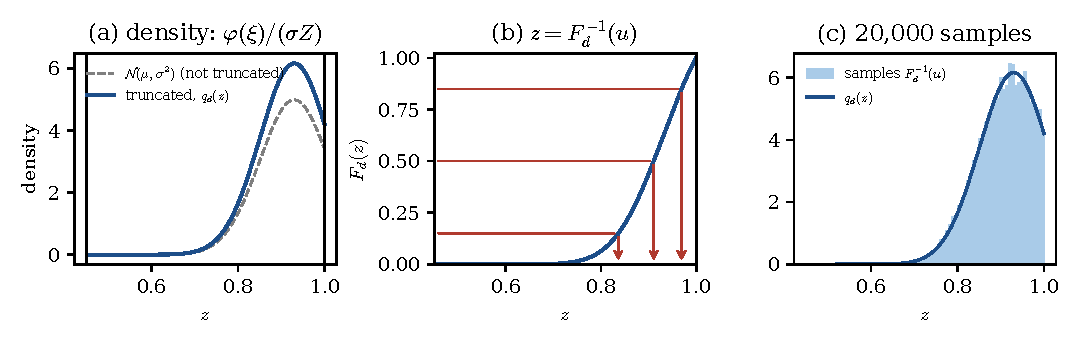
\includegraphics[width=\linewidth]{inverse_cdf.pdf}
\caption{Inverse-CDF sampling of a truncated Gaussian on $[0.45,1]$ ($\mu=0.93$, $\sigma=0.08$). (a) The truncated density is the Gaussian restricted to the interval and divided by the mass $Z$ inside it, so it is higher than the parent density. (b) A uniform level $u$ is mapped to $z=F_d^{-1}(u)$. (c) The samples follow $q_d$, and every sample lies in the interval.}
\label{fig:inverse_cdf}
\end{figure}

\subsection{Sklar's theorem and the copula density}
\begin{definition}
A $D$-dimensional copula is the joint CDF of a random vector $\uu=(U_1,\dots,U_D)$ whose marginals are all $\U(0,1)$:
\begin{equation*}
C(u_1,\dots,u_D)=P(U_1\le u_1,\dots,U_D\le u_D).
\end{equation*}
\end{definition}
\begin{proposition}[Sklar \cite{sklar1959,nelsen2006}, continuous case]
Let $\z$ have joint CDF $F_{\z}$ and continuous, strictly increasing marginal CDFs $F_1,\dots,F_D$. Then there is a copula $C$ such that
\begin{equation}
F_{\z}(z_1,\dots,z_D)=C\big(F_1(z_1),\dots,F_D(z_D)\big).
\label{eq:sklar}
\end{equation}
Conversely, for any copula $C$ and any continuous marginal CDFs, \eqref{eq:sklar} defines a joint CDF with those marginals.
\end{proposition}
\begin{proof}
Let $U_d=F_d(z_d)$. By Lemma~\ref{lem:pit}(i) each $U_d$ is $\U(0,1)$, so the joint CDF $C$ of $(U_1,\dots,U_D)$ is a copula. Since every $F_d$ is increasing, $z_d\le t_d$ iff $U_d\le F_d(t_d)$, and $F_{\z}(\mathbf t)=P(U_1\le F_1(t_1),\dots,U_D\le F_D(t_D))=C(F_1(t_1),\dots,F_D(t_D))$.
Conversely, let $\uu$ have CDF $C$ and $z_d=F_d^{-1}(u_d)$. Then $z_d\le t_d$ iff $u_d\le F_d(t_d)$, so the joint CDF of $\z$ is $C(F_1(t_1),\dots)$, and its $d$-th marginal is $F_d$ by Lemma~\ref{lem:pit}(ii).
\end{proof}
The copula carries all the dependence; the marginals carry everything else (location, spread, skewness, bounds, modes). This separation is what makes copulas useful for VI \cite{tran2015copula}: the marginals and the dependence can be chosen separately.

\paragraph{The joint density.} The density is the mixed derivative of the CDF, $q(\z)=\partial^DF_{\z}/\partial z_1\cdots\partial z_D$. In $C(F_1(z_1),\dots,F_D(z_D))$, each argument depends on one variable only, so each derivative $\partial/\partial z_d$ acts on the $d$-th argument and produces, by the chain rule, a factor $F_d'(z_d)=q_d(z_d)$:
\begin{equation}
q(\z)=c\big(F_1(z_1),\dots,F_D(z_D)\big)\prod_{d=1}^Dq_d(z_d),\qquad c(\uu)=\frac{\partial^DC(\uu)}{\partial u_1\cdots\partial u_D},
\label{eq:copula_joint}
\end{equation}
where $c$ is the copula density. With independent components, $C(\uu)=\prod_du_d$, $c\equiv1$, and $q$ is the product of its marginals (mean field).

\subsection{The Gaussian copula}
The Gaussian copula is the copula of a Gaussian vector $\y\sim\N(\mathbf0,\Sig)$ whose covariance $\Sig$ has unit diagonal (a correlation matrix), so that each $y_d$ is $\N(0,1)$ (Proposition~\ref{prop:mvn_linear}(a)). Its uniforms are $u_d=\Psi(y_d)$.

\begin{proposition}[Gaussian copula model: sampling and density]
\label{prop:copula_sampling}
Let $\eps\sim\N(\mathbf0,\I)$, $\y=\Lb\eps$ with $\Lb\Lb^\top=\Sig$ a correlation matrix, $u_d=\Psi(y_d)$, and $z_d=F_d^{-1}(u_d)$, where each $F_d$ is a continuous CDF with density $q_d$. Then:
(i) $\y\sim\N(\mathbf0,\Sig)$; (ii) each $u_d\sim\U(0,1)$ and each $z_d$ has density $q_d$; (iii) $\z$ has the joint density
\begin{equation}
\begin{gathered}
\qth(\z)=c_{\Sig}(\uu)\prod_{d=1}^Dq_d(z_d),\qquad
c_{\Sig}(\uu)=|\Sig|^{-1/2}\exp\Big(-\tfrac12\,\y^\top\big(\Sig^{-1}-\I\big)\y\Big),\\
y_d=\Psi^{-1}(u_d),\qquad u_d=F_d(z_d).
\end{gathered}
\label{eq:gauss_copula_density}
\end{equation}
\end{proposition}
\begin{proof}
(i) Proposition~\ref{prop:mvn}(ii).
(ii) $y_d\sim\N(0,\Sigma_{dd})=\N(0,1)$ by Proposition~\ref{prop:mvn_linear}(a), so $u_d=\Psi(y_d)\sim\U(0,1)$ by Lemma~\ref{lem:pit}(i), and $z_d=F_d^{-1}(u_d)$ has CDF $F_d$ by Lemma~\ref{lem:pit}(ii).
(iii) The map $\z\mapsto\y$, $y_d=\Psi^{-1}(F_d(z_d))$, acts componentwise, so its Jacobian is diagonal. Differentiating $\Psi(y_d)=F_d(z_d)$ with respect to $z_d$ gives $\varphi(y_d)\,\frac{\dd y_d}{\dd z_d}=q_d(z_d)$, i.e., $\frac{\dd y_d}{\dd z_d}=\frac{q_d(z_d)}{\varphi(y_d)}$. By Theorem~\ref{thm:cov_multi} (the density of $\z$ is the density of $\y$ times the Jacobian determinant of $\z\mapsto\y$),
\begin{equation*}
\qth(\z)=\varphi_{\Sig}(\y)\prod_d\frac{q_d(z_d)}{\varphi(y_d)}=\frac{\varphi_{\Sig}(\y)}{\prod_d\varphi(y_d)}\prod_dq_d(z_d).
\end{equation*}
With~\eqref{eq:mvn} and $\prod_d\varphi(y_d)=(2\pi)^{-D/2}\exp(-\tfrac12\y^\top\y)$ (Proposition~\ref{prop:mvn}(i)),
\begin{equation*}
\frac{\varphi_{\Sig}(\y)}{\prod_d\varphi(y_d)}=\frac{(2\pi)^{-D/2}|\Sig|^{-1/2}\exp(-\tfrac12\y^\top\Sig^{-1}\y)}{(2\pi)^{-D/2}\exp(-\tfrac12\y^\top\y)}=|\Sig|^{-1/2}\exp\Big(-\tfrac12\y^\top(\Sig^{-1}-\I)\y\Big).
\end{equation*}
\end{proof}
The factors $(2\pi)^{-D/2}$ cancel, so the prefactor of $c_{\Sig}$ is $|\Sig|^{-1/2}$.\footnote{Some texts, including Eqs.~(29) and (31) of \cite{fernandez2026pem}, write the prefactor as $1/\sqrt{2\pi|\Sig|}$. The extra $2\pi$ is a constant: it shifts $\log q$ by $-\tfrac12\log2\pi$ and changes neither the minimizer nor the gradients.}
The log-density of the joint model, needed to evaluate $\qth$ at any point $\z$, is
\begin{equation}
\log\qth(\z)=-\tfrac12\log|\Sig|-\tfrac12\,\y^\top(\Sig^{-1}-\I)\y+\sum_{d=1}^D\log q_d(z_d),\qquad y_d=\Psi^{-1}\big(F_d(z_d)\big).
\end{equation}

\begin{procedure}[Sampling the Gaussian copula model]
\label{alg:copula_sampling}
Given $\Lb$ and the marginals $\{F_d\}$: (1) draw $\eps\sim\N(\mathbf0,\I_D)$; (2) correlate, $\y=\Lb\eps$; (3) map to uniforms, $u_d=\Psi(y_d)$; (4) map to the marginals, $z_d=F_d^{-1}(u_d)$.
By Proposition~\ref{prop:copula_sampling}, $\z$ has the density~\eqref{eq:gauss_copula_density}. Every step is a differentiable function of the encoder outputs, so $\z=T_{\thetab}(\eps)$ is a valid reparameterization (Section~\ref{sec:reparam}). If the marginals are truncated to $[\zlb,\zub]$, every sample lies in $\Sset$; no rejection is needed.
\end{procedure}

\paragraph{Parameterization of $\Sig$.} The encoder outputs the $D(D-1)/2$ entries below the diagonal of a lower-triangular matrix $\tilde\Lb$ (linear activation) and its $D$ diagonal entries (softplus, hence positive). Each row is divided by its Euclidean norm, $\Lb_{d,:}=\tilde\Lb_{d,:}/\|\tilde\Lb_{d,:}\|$. Then:
\begin{itemize}
\item $\Sigma_{dd}=(\Lb\Lb^\top)_{dd}=\|\Lb_{d,:}\|^2=1$: $\Sig$ is a correlation matrix;
\item $\Lb$ is triangular with positive diagonal, so $\det\Lb=\prod_dL_{dd}>0$; for $\x\neq\mathbf0$, $\x^\top\Sig\x=\|\Lb^\top\x\|^2>0$ because $\Lb^\top$ is invertible: $\Sig$ is SPD;
\item $\Lb$ is the Cholesky factor of $\Sig$, and $\log|\Sig|=2\sum_d\log L_{dd}$ costs nothing;
\item initializing the weights of the off-diagonal head to zero gives $\tilde\Lb$ diagonal, hence $\Sig=\I$ (independent components) at the start of the training.
\end{itemize}

\paragraph{What the correlation means.} $\Sigma_{de}$ is the correlation of $y_d$ and $y_e$, not of $z_d$ and $z_e$. Each $z_d$ is an increasing function of $y_d$ (a composition of the increasing functions $\Psi$ and $F_d^{-1}$), so: if $\Sigma_{de}>0$, large $z_d$ tend to occur with large $z_e$; if $\Sigma_{de}<0$, with small $z_e$ (the ridge of Example~\ref{ex:2d}); if $\Sig$ is diagonal, the $y_d$ are independent (Corollary~\ref{cor:uncorrelated}), and so are the $z_d$, as functions of independent variables. In the space of $\y$, the joint posterior is a Gaussian ellipsoid; in $\z$, it is that ellipsoid deformed componentwise by the marginals (Fig.~\ref{fig:copula_marginals}). The Gaussian copula therefore cannot represent dependence whose direction changes across the domain (e.g., a curved ridge that bends back), nor modes in arbitrary positions \cite{joe2014}.

\begin{figure}[t]
\centering
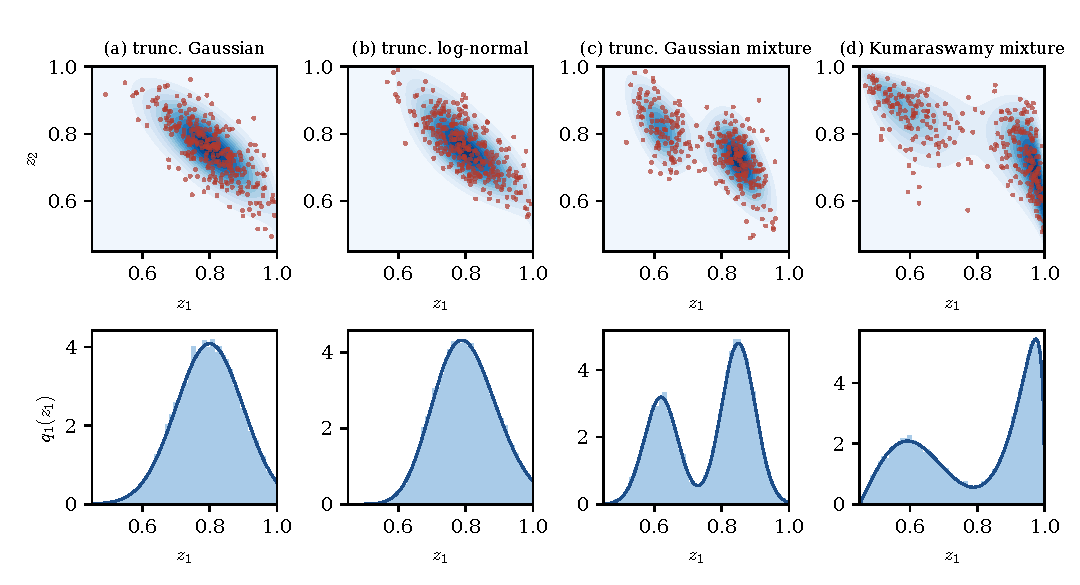
\includegraphics[width=\linewidth]{copula_marginals.pdf}
\caption{The same Gaussian copula ($\Sigma_{12}=-0.75$) with four marginal families on $[0.45,1]$. Top: joint density~\eqref{eq:gauss_copula_density} (blue) and 300 samples of Algorithm~\ref{alg:copula_sampling} (red). Bottom: marginal density of $z_1$ and histogram of 20,000 samples. (a) Truncated Gaussian; (b) truncated log-normal; (c) two-component truncated Gaussian mixture for $z_1$; (d) two-component Kumaraswamy mixture for $z_1$.}
\label{fig:copula_marginals}
\end{figure}

% -----------------------------------------------------------------------------------------------------
\section{Marginal families}
\label{sec:marginals}
For each family we derive the density, the CDF, the inverse CDF (needed by Algorithm~\ref{alg:copula_sampling}), the entropy (needed by the loss), the mean (the point estimate) and the probability of damage $P_d=F_d(\tau)$.

\subsection{Family A: truncated Gaussian}
\label{sec:tn}
\paragraph{Definition by conditioning.} Let $X\sim\N(\mu,\sigma^2)$ (the parent Gaussian) and restrict it to $[\zlb,\zub]$: the truncated variable has the distribution of $X$ conditioned on $\zlb\le X\le\zub$. For $z$ in the interval, the conditional density is the parent density divided by the probability of the condition (definition of conditional probability):
\begin{equation*}
q(z)=\frac{p_X(z)}{P(\zlb\le X\le\zub)}.
\end{equation*}
Define the standardized bounds and the probability of the interval,
\begin{equation}
\xi=\frac{z-\mu}{\sigma},\qquad\alpha=\frac{\zlb-\mu}{\sigma},\qquad\beta=\frac{\zub-\mu}{\sigma},\qquad Z=P(\zlb\le X\le\zub)=\Psi(\beta)-\Psi(\alpha).
\end{equation}
With $p_X(z)=\varphi(\xi)/\sigma$ (Eq.~\eqref{eq:gauss_pdf}):
\begin{equation}
q(z)=\frac{\varphi(\xi)}{\sigma Z},\qquad z\in[\zlb,\zub],\qquad q(z)=0\ \text{otherwise}.
\end{equation}
$\mu$ and $\sigma$ are the location and scale of the parent, not the mean and standard deviation of the truncated variable. The location may lie outside the interval: a healthy component has $\mu\ge\zub$, and its density increases up to $z=1$ (Fig.~\ref{fig:inverse_cdf}a).

\paragraph{CDF.} For $z\in[\zlb,\zub]$, with the substitution $t=\mu+\sigma\xi'$:
\begin{equation}
F(z)=\int_{\zlb}^z\frac{\varphi((t-\mu)/\sigma)}{\sigma Z}\dd t=\frac1Z\int_\alpha^\xi\varphi(\xi')\dd\xi'=\frac{\Psi(\xi)-\Psi(\alpha)}{Z}.
\end{equation}
It is 0 at $\zlb$ ($\xi=\alpha$) and 1 at $\zub$ ($\xi=\beta$).

\paragraph{Inverse CDF.} Solve $F(z)=u$ for $z$: $\Psi(\xi)=\Psi(\alpha)+uZ$, so $\xi=\Psi^{-1}(\Psi(\alpha)+uZ)$ and
\begin{equation}
z=F^{-1}(u)=\mu+\sigma\,\Psi^{-1}\big(\Psi(\alpha)+u\,Z\big).
\label{eq:tn_quantile}
\end{equation}
It is a closed-form, differentiable function of $u$, $\mu$ and $\sigma$.

\paragraph{Numerical stability.} If the interval lies in a tail of the parent (e.g., $\mu\gg\zub$), $\Psi(\alpha)$ and $\Psi(\beta)$ are both close to 1; their difference $Z$ and the argument $\Psi(\alpha)+uZ$ lose their significant digits in single precision. The implementation computes $Z=1-\Psi(\alpha)-\Psi(-\beta)$ from the two tails, and, when $\Psi(\alpha)+uZ>0.5$, uses the equivalent equation written for the upper tail. Since $1-\Psi(\xi)=\Psi(-\xi)$ and $1-\Psi(\alpha)=\Psi(-\beta)+Z$,
\begin{equation*}
\Psi(-\xi)=1-\Psi(\alpha)-uZ=\Psi(-\beta)+(1-u)Z\quad\Longrightarrow\quad\xi=-\Psi^{-1}\big(\Psi(-\beta)+(1-u)Z\big),
\end{equation*}
so that $\Psi^{-1}$ never receives an argument of the form $1-\text{tiny}$.

\begin{proposition}[Moments]
\label{prop:tn_moments}
With $\xi$ the standard normal truncated to $[\alpha,\beta]$ (density $\varphi(\xi)/Z$ there),
\begin{equation}
\E[\xi]=\frac{\varphi(\alpha)-\varphi(\beta)}{Z},\qquad\E[\xi^2]=1+\frac{\alpha\varphi(\alpha)-\beta\varphi(\beta)}{Z},
\end{equation}
and, since $z=\mu+\sigma\xi$, $\E[z]=\mu+\sigma\,\frac{\varphi(\alpha)-\varphi(\beta)}{Z}$ and $\Var[z]=\sigma^2(\E[\xi^2]-\E[\xi]^2)$.
\end{proposition}
\begin{proof}
Use $\xi\varphi(\xi)=-\varphi'(\xi)$ (Section~\ref{sec:gauss}). First, $\int_\alpha^\beta\xi\varphi\dd\xi=[-\varphi]_\alpha^\beta=\varphi(\alpha)-\varphi(\beta)$. Second, by parts with $f=\xi$ and $g'=\xi\varphi=-\varphi'$:
$\int_\alpha^\beta\xi^2\varphi\dd\xi=[-\xi\varphi]_\alpha^\beta+\int_\alpha^\beta\varphi\dd\xi=\alpha\varphi(\alpha)-\beta\varphi(\beta)+Z$. Divide both by $Z$.
\end{proof}
The mean is below $\mu$ when the upper bound cuts more than the lower one ($\varphi(\beta)>\varphi(\alpha)$), as in Example~\ref{ex:1d}.

\paragraph{Entropy.} $\log q(z)=-\log(\sigma Z)-\tfrac12\log(2\pi)-\tfrac12\xi^2$, so, with Proposition~\ref{prop:tn_moments},
\begin{equation}
\Hent[q]=\log(\sigma Z)+\tfrac12\log(2\pi)+\tfrac12\E[\xi^2]
=\log\big(\sqrt{2\pi e}\,\sigma Z\big)+\frac{\alpha\varphi(\alpha)-\beta\varphi(\beta)}{2Z},
\label{eq:tn_entropy}
\end{equation}
where $\tfrac12\log(2\pi)+\tfrac12=\log\sqrt{2\pi e}$. Without truncation ($Z\to1$, $\alpha\to-\infty$, $\beta\to\infty$) this is the Gaussian entropy $\log(\sqrt{2\pi e}\sigma)$.

\paragraph{Unit-space parameterization.} The revised code (family GC-TN) defines the truncated Gaussian for $x\in[0,1]$ and maps $z=\zlb+(\zub-\zlb)x$. By Lemma~\ref{lem:entropy_cov}, $\Hent[z]=\Hent[x]+\log(\zub-\zlb)$. The location is a sigmoid output in $(0,1)$ and the scale lies in $(10^{-3},5)$.

\paragraph{Probability of damage.} $P_d=F(\tau)=\big(\Psi((\tau-\mu)/\sigma)-\Psi(\alpha)\big)/Z$.

\subsection{Family B: truncated log-normal (the model of the revised manuscript)}
\label{sec:logn}
Let $w=\log z$ follow a Gaussian with location $m$ and scale $s$ truncated to $[\log\zlb,\log\zub]=[\log\zlb,0]$ (family A in the variable $w$), with $\alpha=(\log\zlb-m)/s$, $\beta=(0-m)/s$, $Z=\Psi(\beta)-\Psi(\alpha)$.

\paragraph{Density, CDF, inverse CDF.} The map $z=e^w$ is increasing with $\dd z/\dd w=e^w=z$; by Proposition~\ref{prop:cov1d}, $q_z(z)=q_w(\log z)/z$:
\begin{equation}
q(z)=\frac{\varphi\big((\log z-m)/s\big)}{s\,Z\,z},\qquad z\in[\zlb,1].
\end{equation}
Since $z\le t$ iff $w\le\log t$, $F_z(t)=F_w(\log t)$, and $F_z^{-1}(u)=\exp(F_w^{-1}(u))$:
\begin{equation}
F(z)=\frac{\Psi\big((\log z-m)/s\big)-\Psi(\alpha)}{Z},\qquad
F^{-1}(u)=\exp\Big(m+s\,\Psi^{-1}\big(\Psi(\alpha)+uZ\big)\Big).
\end{equation}
The same tail-stable evaluation as in family A applies to the inner quantile.

\paragraph{Mean.} With $w=m+s\xi$, $\E[z]=\E[e^{m+s\xi}]$ with $\xi$ truncated to $[\alpha,\beta]$. Completing the square in the exponent, $m+s\xi-\tfrac12\xi^2=m+\tfrac12s^2-\tfrac12(\xi-s)^2$, so $e^{m+s\xi}\varphi(\xi)=e^{m+s^2/2}\varphi(\xi-s)$, and
\begin{equation}
\E[z]=\frac1Z\int_\alpha^\beta e^{m+s\xi}\varphi(\xi)\dd\xi=\frac{e^{m+s^2/2}}{Z}\int_{\alpha-s}^{\beta-s}\varphi(t)\dd t=e^{m+s^2/2}\,\frac{\Psi(\beta-s)-\Psi(\alpha-s)}{Z}.
\end{equation}

\paragraph{Entropy.} By Lemma~\ref{lem:entropy_cov} with $g(w)=e^w$, $\Hent[z]=\Hent[w]+\E[w]$; $\Hent[w]$ is~\eqref{eq:tn_entropy} with $(s,\alpha,\beta,Z)$, and $\E[w]=m+s\E[\xi]$ by Proposition~\ref{prop:tn_moments}:
\begin{equation}
\Hent[z]=\log\big(\sqrt{2\pi e}\,s\,Z\big)+\frac{\alpha\varphi(\alpha)-\beta\varphi(\beta)}{2Z}+m+s\,\frac{\varphi(\alpha)-\varphi(\beta)}{Z}.
\end{equation}

\paragraph{Probability of damage.} $P_d=F(\tau)=\big(\Psi((\log\tau-m)/s)-\Psi(\alpha)\big)/Z$.

\paragraph{Why the log scale.} The marginals of the exact posteriors are right-skewed in $z$ (a longer tail towards low stiffness) and nearly symmetric in $\log z$. One reason: the natural frequencies of a structure whose stiffness is scaled by $z$ scale as $\sqrt z$ (the eigenvalues $\omega^2$ of $z\mathbf K\bm\phi=\omega^2\mathbf M\bm\phi$ are $z$ times those of $\mathbf K\bm\phi=\omega^2\mathbf M\bm\phi$), so $\log f=\tfrac12\log z+\text{const}$; for local damage the dependence is not exactly linear but remains smooth in $\log z$. A Gaussian error in $\log f$ (Example~\ref{ex:multiplicative}) then gives a nearly Gaussian likelihood in $\log z$ (Example~\ref{ex:1d} with $\log z$ in place of $z$). One Gaussian component in $\log z$ follows these marginals better than one in $z$, with the same number of parameters. The location is allowed in $(\log\zlb-3s,\ 3s)$, so the peak of the parent may lie up to three scales outside the support, and the density may increase up to $z=1$ (healthy components).

\begin{remark}
The run of the revised manuscript (\texttt{GCLogN\_13Nov-DoE30\_7D\_}\allowbreak\texttt{Gamma1.0\_Conv6000}) uses this family. The revised manuscript, however, writes the formulas of family A (truncated Gaussian in $z$) for the marginals, the quantile and the posterior mean of its appendix. The formulas of the trained model are those of this section.
\end{remark}

\subsection{Family C: truncated Gaussian mixtures}
\label{sec:gm}
A marginal can be a mixture of $K$ truncated Gaussian components (family A) with weights $w_k\ge0$, $\sum_kw_k=1$ (softmax output of the encoder):
\begin{equation}
q(z)=\sum_{k=1}^Kw_k\,\frac{\varphi(\xi_k)}{\sigma_kZ_k},\qquad
F(z)=\sum_{k=1}^Kw_k\,\frac{\Psi(\xi_k)-\Psi(\alpha_k)}{Z_k},\qquad\xi_k=\frac{z-\mu_k}{\sigma_k}.
\end{equation}
Each component integrates to one on the interval, so $\int q=\sum_kw_k=1$; the CDF is the same weighted sum of the component CDFs (the integral is linear).
Truncating each component and then mixing is equivalent to truncating the untruncated mixture with modified weights: $\big(\sum_kw_kp_k\ind\big)/\big(\sum_jw_jZ_j\big)=\sum_k\frac{w_kZ_k}{\sum_jw_jZ_j}\cdot\frac{p_k\ind}{Z_k}$, where $p_k$ is the parent density of component $k$.

\paragraph{Inverse CDF.} $F$ is a sum of CDFs and has no closed-form inverse. It is continuous and strictly increasing on the interval, from 0 to 1, so $F(z)=u$ has exactly one root, found by bisection: start from $[\zlb,\zub]$ and halve the interval, keeping the half where $F-u$ changes sign; each halving divides the error by 2, and 60 halvings reach machine precision. Newton's method, safeguarded by bisection, is faster. The derivative of the root follows from~\eqref{eq:implicit_grad}.
This is the main cost of mixture marginals in a copula model: every sample requires one root finding per dimension. Sampling a mixture by first drawing the component index is not an option: the copula needs the quantile $F^{-1}(u_d)$ of the whole marginal at the level $u_d$ given by the copula, and a discrete index cannot be reparameterized.

\paragraph{Entropy.} The entropy of a mixture has no closed form. By Lemma~\ref{lem:pit}, $z=F^{-1}(u)$ with $u\sim\U(0,1)$ has density $q$, so $\Hent[q]=-\E_{u}[\log q(F^{-1}(u))]\approx-\frac1H\sum_h\log q(F^{-1}(u^h))$. The uniforms $u_d^h$ of the copula can be reused with their gradient stopped: each $u_d$ is $\U(0,1)$ whatever $\Sig$ (Proposition~\ref{prop:copula_sampling}(ii)), so the estimate is unbiased for the marginal entropy; stopping the gradient prevents the copula parameters from receiving a spurious gradient from the marginal entropy (the copula part is exact,~\eqref{eq:copula_entropy}).

\paragraph{Mean and probability of damage.} Weighted sums of the component values: $\E[z]=\sum_kw_k\E_k[z]$ (Proposition~\ref{prop:tn_moments} for each component) and $P_d=F(\tau)$.

\paragraph{Behavior.} Mixtures capture multimodal marginals (``$z_1$ is either mildly or severely damaged''). With the Gaussian copula (Fig.~\ref{fig:copula_marginals}c), the joint density becomes multimodal, but its modes are not free: they are images of the same Gaussian ellipsoid through the marginal maps, so they lie on a grid aligned with the coordinate axes and share the same dependence. Two modes in different directions (``zone 1 or bearing L damaged'') require a joint mixture, not a mixture in the marginals. Mixtures also bring label switching (permuting the components gives the same density) and components that collapse onto each other; the number of parameters is $3K-1$ per dimension.

\subsection{Family D: Kumaraswamy and Kumaraswamy mixtures}
\label{sec:ks}
The Kumaraswamy distribution \cite{kumaraswamy1980} on $x\in[0,1]$, with $a,b>0$, is defined by its CDF $F(x)=1-(1-x^a)^b$, which increases from $F(0)=0$ to $F(1)=1$. Its density is the derivative (chain rule):
\begin{equation}
q(x)=F'(x)=b(1-x^a)^{b-1}\cdot ax^{a-1}=a\,b\,x^{a-1}(1-x^a)^{b-1}.
\end{equation}
The inverse CDF follows from $1-(1-x^a)^b=u$: $(1-x^a)^b=1-u$, $x^a=1-(1-u)^{1/b}$, so
\begin{equation}
F^{-1}(u)=\big(1-(1-u)^{1/b}\big)^{1/a}.
\end{equation}
It is bounded by construction (no truncation needed) and, unlike the Beta distribution, has closed-form CDF and quantile. The map $z=\zlb+(\zub-\zlb)x$ places it on the prior interval and adds $\log(\zub-\zlb)$ to the entropy (Lemma~\ref{lem:entropy_cov}). With $a<1$ (resp.\ $b<1$) the density tends to infinity at $x=0$ (resp.\ $x=1$), which can represent a posterior piled against $z=1$. A mixture of Kumaraswamy components (Fig.~\ref{fig:copula_marginals}d) keeps the closed-form CDF, but, as for Gaussian mixtures, its quantile requires root finding and its entropy requires Monte Carlo. Numerically, $\log(1-x^a)$ must be computed as $\log\big(-\mathrm{expm1}(a\log x)\big)$, where $\mathrm{expm1}(t)=e^t-1$ is evaluated without cancellation: for $x$ close to 1, $x^a$ is close to 1 and $1-x^a$ would lose its digits.

\subsection{Comparison of the families}
\begin{table}[h]
\centering
\caption{Marginal families in the Gaussian copula model ($K$: number of components; $^*$closed form for $K=1$).}
\label{tab:families}
\small
\begin{tabular}{@{}lccccc@{}}
\toprule
Family & bounded & CDF & quantile & entropy & param./dim. \\
\midrule
A: trunc.\ Gaussian & truncation & closed & closed & closed & 2 \\
B: trunc.\ log-normal & truncation & closed & closed & closed & 2 \\
C: trunc.\ Gaussian mixture & truncation & closed & root finding & Monte Carlo & $3K-1$ \\
D: Kumaraswamy mixture & yes & closed & root finding$^*$ & Monte Carlo & $3K-1$ \\
\bottomrule
\end{tabular}
\end{table}
The copula adds $D(D-1)/2$ parameters in every case. For comparison, a joint Gaussian mixture with full covariances needs $(K-1)$ weights, $KD$ means and $KD(D+1)/2$ covariance entries, i.e., $K(1+D+D(D+1)/2)-1$ parameters, and, when truncated to the box, the normalizer $C(\thetab)=\int_{\Sset} q$, which has no closed form \cite{fernandez2026pem}. The copula with families A or B needs $2D+D(D-1)/2$ parameters and no normalizer.

\subsection{Truncation: summary}
\begin{itemize}
\item \emph{Why truncate.} The prior is zero outside $\Sset$, so any $q$ with mass outside $\Sset$ has an infinite KL divergence from the posterior (Section~\ref{sec:kl}); physically, $z>1$ and $z<\zlb$ are excluded by the model.
\item \emph{How.} Put the truncation in the density (normalizer $Z$), in the CDF and in the quantile. Inverse-CDF sampling then gives valid samples with an exactly known density.
\item \emph{What to avoid.} Clipping (atoms at the bounds), rejection without the normalizer and without accounting for its effect on the gradient (Section~\ref{sec:rejection}), and penalties that push samples away from the bounds (they bias the healthy components).
\end{itemize}

% =====================================================================================================
\section{One training step, from the data to the gradient}
\label{sec:step}
For a mini-batch of observations $\{\m_i\}$ and family B (GC-LogN):
\begin{enumerate}
\item \emph{Encoder:} $\mathcal E_{\thetab}(\m_i)\mapsto\{m_{i,d},s_{i,d}\}_{d=1}^D$, the $D(D-1)/2$ off-diagonal entries and the $D$ diagonal entries of $\tilde\Lb_i$; row-normalize to obtain $\Lb_i$.
\item \emph{Sampling} (Algorithm~\ref{alg:copula_sampling}): $\eps_i^h\sim\N(\mathbf0,\I)$, $\y_i^h=\Lb_i\eps_i^h$, $u_{i,d}^h=\Psi(y_{i,d}^h)$, and
\begin{equation*}
z_{i,d}^h=\exp\Big(m_{i,d}+s_{i,d}\Psi^{-1}\big(\Psi(\alpha_{i,d})+u_{i,d}^hZ_{i,d}\big)\Big).
\end{equation*}
\item \emph{Decoder:} assemble $\mathbf K_{\text G}(\z_i^h)=\sum_ez_e\mathbf K_e$, solve the eigenvalue problem, extract $\hat{\mathbf f}(\z_i^h)$ and $\hat{\bm\Phi}(\z_i^h)$ at the sensors.
\item \emph{Likelihood:} $\NLL(\z_i^h;\m_i)$, Eq.~\eqref{eq:nll_revised}.
\item \emph{Entropy:} $\Hent[q_i]=\sum_d\Hent[q_{i,d}]+\sum_d\log L_{i,dd}$ in closed form (Section~\ref{sec:logn} and Proposition~\ref{prop:copula_entropy}).
\item \emph{Loss:} Eq.~\eqref{eq:revised_loss}, with the factor $\tau$ on the NLL during the warm-up.
\item \emph{Gradient:} automatic differentiation through the entropy (closed form), the decoder (eigensolver) and the sampler (closed-form quantile); Adam update of $\thetab$.
\end{enumerate}
At inference, steps 1 and 2 give the posterior of a new observation; the decoder is not needed. The marginal summaries (mean, quantiles, $P_d$) follow in closed form from $\{m_d,s_d\}$, and the joint density, if needed, from $\Lb$.

% =====================================================================================================
\section{Self-check questions}
\begin{enumerate}
\item Why does the loss not contain $\z^{\text{true}}$, and what would change if we added $\|\z-\z^{\text{true}}\|^2$? \\
\emph{It would no longer be an ELBO: the minimizer would be pulled towards a regression estimate, and the width of $q$ would no longer be the posterior width.}
\item The data are made twice as noisy, but the variances in the NLL are not changed. What happens to the estimated posterior? \\
\emph{It stays as narrow as before, while the true posterior doubles its width (Example~\ref{ex:1d}: $s=\sigma/a$): overconfident intervals, equivalent to $\gamma=0.5$ for the true error model.}
\item Why is $\E_q[\log p(\z)]$ absent from the code? \\
\emph{With the uniform prior it is the constant $-D\log(\zub-\zlb)$, provided $q$ is supported in $\Sset$.}
\item What does the term $\sum_d\log L_{dd}$ do during training? \\
\emph{It is $\tfrac12\log|\Sig|\le0$ (Lemma~\ref{lem:hadamard}); with the minus sign in the loss, it penalizes correlation, so the copula becomes correlated only when the data imply a ridge.}
\item Why can the training set contain 30\% healthy structures without biasing the posterior towards healthy values? \\
\emph{Because the prior in the loss is uniform; the composition only weights the regions of the observation space (Proposition~\ref{prop:amortized}).}
\item If the exact posterior is bimodal, what does the copula VAE with unimodal marginals return? \\
\emph{Typically the dominant mode, with intervals that underestimate the uncertainty (reverse KL, Section~\ref{sec:reverse_kl}).}
\item Why can the truncated-Gaussian quantile be differentiated directly, while the mixture quantile needs Eq.~\eqref{eq:implicit_grad}? \\
\emph{The first is a closed formula in $(u,\mu,\sigma)$; the second is the output of a root-finding loop, whose derivative follows from the identity $F(z;\thetab)=u$.}
\item In Example~\ref{ex:1d}, what is the posterior if $\hat z=y/a=1.05$, outside the prior interval? \\
\emph{The truncated Gaussian with location $1.05$: a density increasing up to $z=1$. The data suggest a stiffness slightly above the intact one, which the prior excludes; the posterior puts its mass just below 1.}
\end{enumerate}

% =====================================================================================================
\begin{thebibliography}{99}\small
\bibitem{bishop2006} C.~M. Bishop, \emph{Pattern Recognition and Machine Learning}, Springer, 2006 (Chapters~2 and~10).
\bibitem{bissiri2016general} P.~G. Bissiri, C.~C. Holmes, S.~G. Walker, A general framework for updating belief distributions, \emph{J. R. Stat. Soc. B} 78(5) (2016) 1103--1130.
\bibitem{blei2017vi} D.~M. Blei, A. Kucukelbir, J.~D. McAuliffe, Variational inference: a review for statisticians, \emph{J. Am. Stat. Assoc.} 112(518) (2017) 859--877.
\bibitem{cover2006} T.~M. Cover, J.~A. Thomas, \emph{Elements of Information Theory}, 2nd ed., Wiley, 2006.
\bibitem{cremer2018} C. Cremer, X. Li, D. Duvenaud, Inference suboptimality in variational autoencoders, \emph{ICML} 2018.
\bibitem{delmoral2006smc} P. Del Moral, A. Doucet, A. Jasra, Sequential Monte Carlo samplers, \emph{J. R. Stat. Soc. B} 68(3) (2006) 411--436.
\bibitem{fernandez2026pem} A. Fern\'andez-Navamuel, M.~A. D\'iaz Viera, M. Croci, A copula-based variational autoencoder for uncertainty quantification in inverse structural dynamics: application to damage identification in an offshore wind turbine, \emph{Probab. Eng. Mech.} 86 (2026) 104054.
\bibitem{figurnov2018implicit} M. Figurnov, S. Mohamed, A. Mnih, Implicit reparameterization gradients, \emph{NeurIPS} 2018.
\bibitem{higgins2017beta} I. Higgins et al., $\beta$-VAE: learning basic visual concepts with a constrained variational framework, \emph{ICLR} 2017.
\bibitem{joe2014} H. Joe, \emph{Dependence Modeling with Copulas}, CRC Press, 2014.
\bibitem{kingma2014vae} D.~P. Kingma, M. Welling, Auto-encoding variational Bayes, \emph{ICLR} 2014.
\bibitem{kullback1951} S. Kullback, R.~A. Leibler, On information and sufficiency, \emph{Ann. Math. Stat.} 22(1) (1951) 79--86.
\bibitem{kumaraswamy1980} P. Kumaraswamy, A generalized probability density function for double-bounded random processes, \emph{J. Hydrol.} 46 (1980) 79--88.
\bibitem{mohamed2020mcgrad} S. Mohamed, M. Rosca, M. Figurnov, A. Mnih, Monte Carlo gradient estimation in machine learning, \emph{J. Mach. Learn. Res.} 21(132) (2020) 1--62.
\bibitem{nelsen2006} R.~B. Nelsen, \emph{An Introduction to Copulas}, 2nd ed., Springer, 2006.
\bibitem{rezende2014} D.~J. Rezende, S. Mohamed, D. Wierstra, Stochastic backpropagation and approximate inference in deep generative models, \emph{ICML} 2014.
\bibitem{roeder2017sticking} G. Roeder, Y. Wu, D. Duvenaud, Sticking the landing: simple, lower-variance gradient estimators for variational inference, \emph{NeurIPS} 2017.
\bibitem{sklar1959} A. Sklar, Fonctions de r\'epartition \`a $n$ dimensions et leurs marges, \emph{Publ. Inst. Statist. Univ. Paris} 8 (1959) 229--231.
\bibitem{tran2015copula} D. Tran, D.~M. Blei, E.~M. Airoldi, Copula variational inference, \emph{NeurIPS} 2015.
\bibitem{zhang2019advances} C. Zhang, J. B\"utepage, H. Kjellstr\"om, S. Mandt, Advances in variational inference, \emph{IEEE Trans. Pattern Anal. Mach. Intell.} 41(8) (2019) 2008--2026.
\end{thebibliography}

\end{document}
